\part{Results}

%% This part has the 3 chapters related to the main results. Each chapter has the results from one of the papers prepared.
\chapter{Long-term characteristics of solar resource over the Iberian Peninsula}

\begin{abstract}
%     {\color{red}QUÉ HAY AQUÍ:
%     \begin{itemize}
%     \item El estudio se basa en productividad en lugar de en radiación.
%     \item Overview de la radiación en largo plazo. Relacionarlo con la nubosidad, con los aerosoles. 
%     \item Metodología extrapolable para otros estudios en distintas escalas tanto temporales como espaciales. Y también para otras energías.
%     \item cuestiones difíciles: no se ha calculado cv para los periodos climatologicamente estables. ¿Hay variaciones decadales? Wild indica que el recurso debe estudiarse solo con los 10 años anteriores! ver la complementariedad con esto.
%     \end{itemize}}

  % ** En este capítulo se ha elaborado una meodología que puede aplicarse al análisis de cuestiones energéticas relacionadas con el largo plazo y escalas temporales climatológicas. Por ejemplo: el estudio de la variabilidad interanual o decadal de los recursos de energías renovables, así como de la producción eléctrica con éstas tecnologías. El método utiliza técnicas de clustering, lo que permite la evaluación espacial de estas cuestiones. Además, posibilita indagar en estudios de complementariedad de distintas fuentes, gracias a la simplificación de la estructura espacial aplicando las técnicas de agrupamiento.

  % ** Este capítulo contiene una nueva perspectiva para el análisis cuestiones climatológicas relacionadas con la producción renovable: esto implica una manera alternativa de analizar: tendencias de la radiación, tendencias de la producción, relación con patrones atmosféricos, complementariedad etc.

  % ** Se puede analizar la influencia de distintos patrones sinópticos sobre la producción eléctrica con energías renovablesen el área de estudio.

  % ** Se puede analizar la influencia de los modos de circulación en grandes escalas

  % ** Con este trabajo, se puede estudiar si las distintas conclusiones que se han encontrado en relación con el recurso en el área sur de Europa, o PI se observan de manera diferenciada en los clusters de la Península, de tal manera, que esta clasificación sirva para tomar decisiones de gestión de produción o de implantación de plantas futuras. Además, el cálculo de la produción eléctrica potencial, permite ir más allá en la evaluación de ciertas métricas como la variabilidad, ya que muchos de los efectos observados en el recurso, se ven amplificados cuando se hace el cálculo de producción.

  % *** ¿Puede el análisis de clustering encontrar zonas diferenciadas de variabilidad interanual?
  % *** ¿Puede el análisis de clustering encontrar zonas de complementariedad del recurso solar?
  % *** ¿Se observan en las distintas zonas la influencia de patrones sinópticos para las distintas estaciones?
  % *** ¿Se observan en las distintas zonas la influencia de los modos de circulación atmosférica como la NAO?
  % *** ¿Es extrapolable el método a otras zonas?
  
The spatio-temporal characteristics of different renewable resources like solar radiation, wind and precipitation are very different among them and a detailed understanding of each is important for an adequate planning and management of the electricity system. In this chapter, we elaborate a comprehensive methodology to analyse variability and complementarity of PV production that can be applied for long-term energy questions and for climate scales, but it is not limited to those time-scales or to solar resource thanks to the flexibility of the method.\\

The work is focused on solar irradiation as source of energy for photovoltaic (PV) generation over the Iberian Peninsula, IP, and on photovoltaic productivity, which is defined as the amount of energy generated normalized by the installed capacity at each location.  The IP is an interesting site due to the fact that it is a large area with limitations in the interconnectivity with the rest of the European continent. It is also a complex climatic area [] due to its geographical location and its orograhy, which makes it interesting for testing the methodology.\\%  \textbf{A comprehensive methodology to analyze variability and complementarity of solar resource and PV production among sub-regions of this area is developed.}

% The photovoltaic energy yield is defined as kWh per kW installed, which facilitates the comparison among sub-regions and allows a comparison with other renewable energies like solar thermoelectric or wind energy.

% \textbf{The multi-step approach facilitates the spatial evaluation and comparison among areas and it could be applied to different time resolutions, from a short term analysis to climatological perspective as well as a climate change projections analysis.}
The main steps of the method are the application of an objective clustering algorithm for performing a regionalization of the whole domain, the analysis of the temporal variability of solar radiation and photovoltaic energy yield, and the intercomparison of the obtained clusters for examining their complementarity.\\

\textbf{The approach applied in this chapter means a different perpective to analyse the long-term issues in solar resource as the interannual variability, the influence of the large-scale circulation modes, trends or the synoptic patterns related to its variability. The use of the multi-step scheme allows to simplify the spatial analysis and answer the questions from a more applied point of view.}\\

% Dar los principales resultados en el abstract
  
Data from a satellite dataset of 30 years, which is usually considered as the time for defining a climatology, is used inthis chapter and a long-term overview of solar radiation variability is analyzed over the Iberian Peninsula (IP). The spatial distribution and variability of photovoltaic (PV) power yield is calculated for different tracking systems. The variability is analyzed on an interannual time scale, which is relevant for energy supply security and year-to-year price stability. It shows robustness and stability of solar radiation and PV production on average for the whole domain, but with significant differences among clusters that could allow spatial compensation of PV production. The relationship between the variability of solar irradiation and of PV yield is not uniform among the different clusters. Areas where solar irradiation is higher are more sensitive to tracking type.\\

The whole process described in this chapter provides the information of how solar resource and the PV energy yield perform in a limited area and provide the tools to analyze the relationships between sub-areas and their variability. In this sense, this method can be applied for isolated or nearly isolated electric systems located in regions with a variety of climates, or for interconnected systems involving several countries.\\ 

%{\color{red}PRINCIPALES RESULTADOS DE LA IP}  

\end{abstract}  

%\clearpage
\section{Introduction}

%In the past few decades, there has been an increase in the renewable energies installed capacity. Renewable technology prices have decreased rapidly attracting investors to the sector, and political agreements such as the requirements of the European Commission for 2020 are also driving this trend. For photovoltaic (PV) energy a large growing trend is expected in the next years \citep{eurostat2014chap124}. 
% {\color{red} \begin{itemize}
% \item eliminar todo lo que hay en la introducción que sea general y pueda ir en la intro del principio
% \item añadir información sobre la evolución de la fotovoltaica en españa
% \item añadir en la intro pq españa es interesante climatológicamente
% \item añadir pq se utiliza satélite  
% \end{itemize}}


The natural variability of renewable energy resources like solar radiation and wind presents some challenges for the management of electricity systems, which were designed for conventional technologies like nuclear or thermal power plants. For that reason a thorough knowledge and understanding of space-time features of solar radiation is needed. In the case of solar PV energy,  its variability \citep{Widen2015} can be studied from the perspective of the resource or from the perspective of the PV power output, that includes some aspects of the PV generators involved in variability, like inverters or tilted and tracking panels which increase the complexity of the assessment. There are many studies focused on the short-term variability \citep{Zamo.Mestre.ea2014} that analyzed PV production ramps due to changes in solar incident irradiation associated with cloud motion \citep{Cros2014, IEA-PVPS-T14-1.32015}. Also, the smoothing effect that a well-spread site planning has on the PV production is being investigated \citep{Marcos2012, Perpinan.Marcos.ea2013}.\\

Not only short-term scales are important to address renewable resources intermittency but also longer time scales are relevant in order to make the system more efficient and reliable \citep{Davy2012}. Policymakers, transmission system operators and investment companies, need an accurate evaluation of resources availability in present and future climate conditions for their mid and long-term planning. The analysis of interannual variability has a particular importance in order to assess stability of the resource and the financial viability of renewable energy plants \citep{pryor2006inter}, as well as the likelihood of strong electricity price oscillations like the ones associated for example with the large interannual variations of hydroelectric production.\\

Regarding that perspective of long-term variability of solar resources, there are studies focused on long series from stations \citep{Sanchez-Lorenzo2009, Sanchez-Lorenzo2013, vazquez2012interannual} or reanalysis data that identify low frequency changes in solar radiation, as the “dimming” and “brightening” periods \citep{Wild2005}, that show relationship between solar irradiation and anthropogenic aerosols \citep{Nabat2014a}. Some studies examine the influence of large-scale circulation atmospheric modes like the NAO (North Atlantic Oscillation) on solar radiation \citep{Pozo-Vazquez2004, Jerez2013}, while others study the spatial variability instead of the temporal variability \citep{Gueymard.Wilcox2011a}.\\ 

Some authors make use of regionalization techniques for atmospheric variables in order to analyze them from a climatological point of view \citep{Argueso2011} or for solar energy purposes, mainly for operation and short-term assessment \citep{Zagouras2013, Zagouras2014, Zagouras.Pedro.2014}.\\

In this chapter a multi-step scheme that systematizes the time-space comparison of solar irradiation or photovoltaic productivity among sub-regions of the target area is described, taking into account a large set of factors involved in PV production that could affect the variability of photovoltaic energy yield. Spatial complementarity between clusters is analyzed through correlation coefficients of solar irradiation and PV energy yield time series, showing possibilities for compensating PV production shortages in certain clusters.\\

The analysis over the Iberian Peninsula show that most of the results obtain in previous studies can be also seen with this approach. In addition, the methodology allow to give a clearer spatial answer to the questions as well as to sistematize the procedure.\\

%As an implementation example, we have performed a long-term analysis of interannual variability of PV energy yield over the Iberian Peninsula, IP, which has a special interest as a nearly-isolated electrical system with a high solar energy potential and a variety of different climates. The use of satellite data in the case of study is explained due to the fact that in some regions there are not enough well-distributed ground stations with long records of solar irradiation. For this kind of study, where spatial features are important, gridded data from satellites are a high quality alternative data source.

This chapter is organized as follows: in first place, a description of the methodolgy is presented. Each stage of the multi-step scheme is summarized in section \ref{Methods} and explained in more detail in the Methodology chapter. After that, the clustering algorithm is applied to the irradiation over the Iberian Peninsula and main results are shown.\\

\subsection{Methods}

The whole comprehensive scheme followed is represented in figure \ref{fig:multi_step}, showing the 4 stages and procedures that will be explained in detail in the following section.\\

From data of solar irradiation on the horizontal plane as the starting point of the method, the most common variable obtained from different data sources, the scheme will provide different outputs that can be used to evaluate resource and PV production:\\

\begin{itemize}
\item Regionalization of the area to facilitate the spatial analysis.
\item Resource and energy yield aggregated by areas.
\item Interannual variability of the resource and the PV production.
\item Evaluation of the complementarity of the resource and PV production among areas.
\end{itemize}  
 
\begin{figure}[h!]
\centering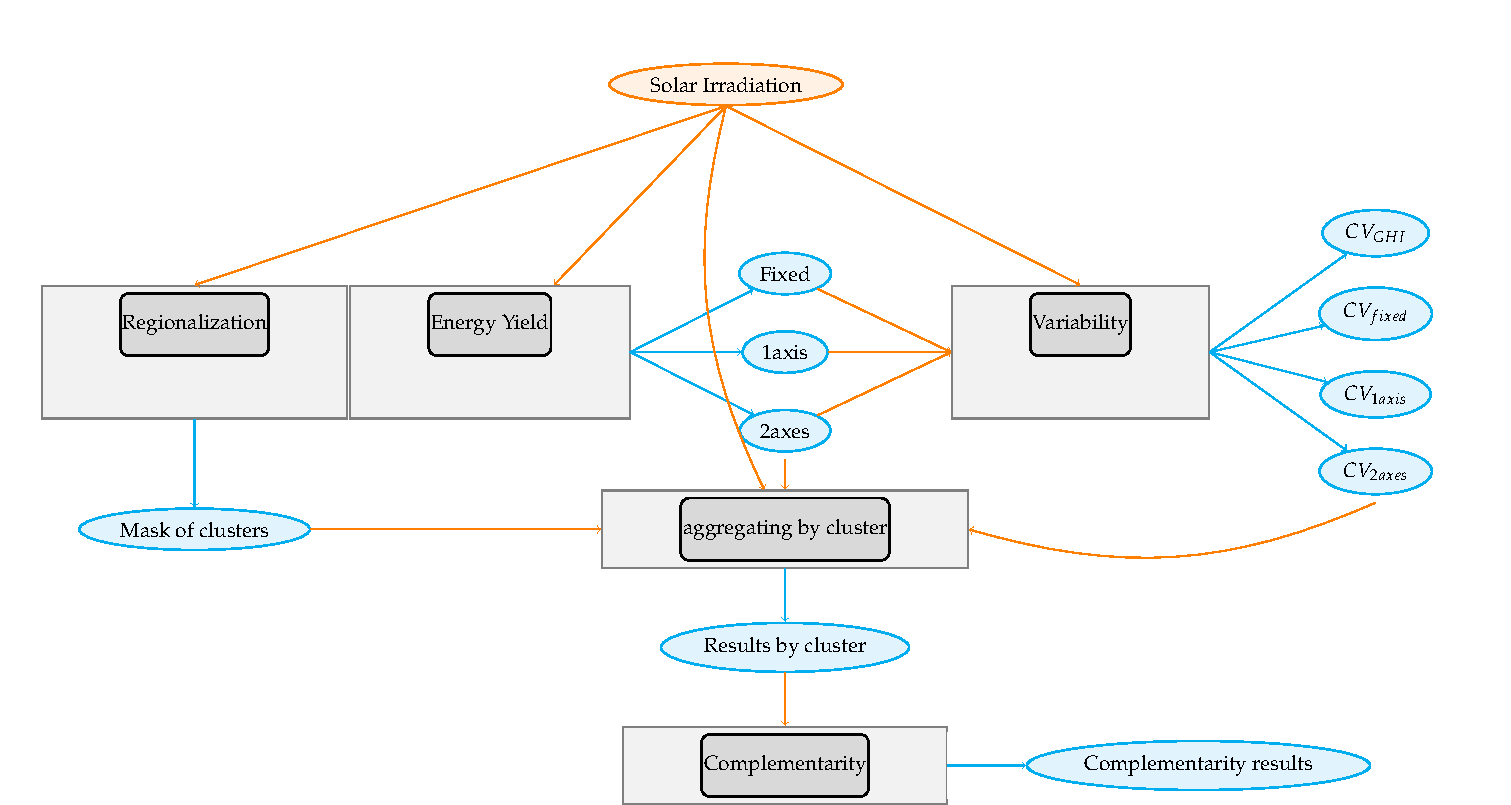
\includegraphics[width=1\textwidth]{figs/capitulo5/multi_step}
\caption{Scheme: Each gray block represents each of the operations needed to get the variability and complementarity results. Orange ellipses are the data employed and blue ellipses are the results of each stage. If the results of one of the blocks are used as input for another stage, connectors are represented in orange color.}
\label{fig:multi_step}
\end{figure}

\subsubsection{Regionalization by clustering}

Regionalization procedures provide the ability of extracting general information of the areas that could be treated as a coherent unit, facilitating the analysis and not considering those characteristics that are not under study. As it was explained in the methodological chapter, classical climatological classifications have some grade of subjectivity due to the fact that they rely on arbitrary assumptions \citep{Kottek2006} and their criteria are based on temperature and precipitation \citep{trewartha1980koppen}. For our purpose, objective and data-derived criteria are more suitable due to the fact that a different variable is analyzed and its classification does not match classical climate divisions. Objective methods based on clustering techniques have been applied successfully over the literature for the analysis of renewable energy resources \citep{Polo2015}, \citep{Zagouras2013}, \citep{Zagouras2014}, \citep{Zagouras.Pedro.2014}, \citep{gomez2015characterization} and atmospheric variables \citep{Argueso2011}, \citep{garcia2012seasonal}. \\

% Clustering methods \citep{Jain1999} can be divided into two categories, partitional and non-partitional. The partitional clustering divides the data into non-overlapping clusters while, the non-partitional or hierarchical clustering, provides a set of nested clusters. In our case, we made use of both algorithms selecting the hierarchical method to initiate a partitional algorithm that is the most suitable for our purpose: to find spatial regions that group together similar time series of the variable analyzed.

A commonly applied regionalization methodology includes the Kmeans algorithm after preprocessing the data through Principal Component Analysis \citep{Ding2004}. This two-step method first reduces redundant information by a Principal Component Analysis that decreases dimensionality of the original dataset. After that, k-means algorithm is applied to the reduced data to find the optimal partition of clusters, which is based on similarity between each element or object inside the cluster and its centroid. This is considered as the most representative element of the cluster, and similarity is measured by an objective function defined in the cluster algorithm.\\

This method presents some problems regarding the random selection of the cluster centroids in the first step. Different initial centroids can lead to different solution or a local optimum could be found. Also, there could be some computational problems if many iterations are needed to get the final partition.\\

The procedure used in \cite{Argueso2011} and in \cite{Zagouras2014} is adapted to get the optimal partition in our scheme from a combined clustering grouping and avoiding the above mentioned problems: the \textbf{k-means partitional algorithm is initialized with a hierarchical clustering solution of a the dimension-reduced data by a Principal Component Analysis.} For the particular case applied in this work, vectors of daily solar irradiation are used for the regionalization. The following steps are needed to get the optimal partition of clusters in the area:\\

\begin{itemize}
\item \textbf{To reduce data dimensionality}. Principal components are eigenvectors of an orthogonal matrix after applied a singular value decomposition (SVD) to the original data, daily solar irradiation vectors, whose initial dimension is reduced to the first eigenvectors that retain $95\%$ of the variance. Considered that, a linear combination of these eigenvectors represents the initial data.
\item \textbf{Hierarchical clustering to initialize k-means}. A hierarchical clustering method classifies data based on a hierarchy. If it is agglomerative, it will start with a cluster for each observation of the data and observations will group together recursively by similarity using the “complete linkage” method. Once the hierarchy is obtained, centroids can be calculated for each emerged partition with a number of clusters between 2 and \textit{n}, where \textit{n} is a high enough selected number of clusters. Centroids will be the initial seed for the Kmeans algorithm, avoiding the computational problems and favoring reproducibility.
\item \textbf{Kmeans algorithm}. The k-means algorithm is a partitional clustering method that minimizes an objective function that defines similarity among the elements of each cluster. In our case we made use of the Euclidean distance, Eq. \ref{eq:euclidean} between the objects or elements in the cluster and its centroid as the objective function. The number of clusters in which the data is divided into has to be known beforehand. In order to overcome the inconvenience, the algorithm is run from 2 to \textit{n} clusters and the optimum number is determined by making use of a clustering validity index after that.
\begin{equation}\label{eq:euclidean}
    J =\sum_{i=1}^{k}\sum_{j=1}^{n}{||x_i-c_j||}^2
\end{equation}


\nomenclature[J]{$J$}{Objective function of the Kmeans clustering method: summation over euclidean distances}
\nomenclature[x_i]{$x_i$}{Each point in the cluster, where the point is a vector with elements comprising the daily irradiation time series values at a pixel obtained from satellite images }
\nomenclature[c_j]{$c_j$}{Centroid of the cluster j}
\nomenclature[PV]{$PV$}{Photovoltaic}
\nomenclature[IP]{$IP$}{Iberian Peninsula}

\item \textbf{Validity index}. In order to determine the optimal partition, validity clustering techniques are applied. There are two types of validation for the clustering methods. First, external clustering validation that make use of external information out of the data; and secondly, there are internal clustering validation methods that rely only on information from the data \citep{5694060}. The latter are used to preserve objectivity as much as possible and are based on two criteria: compactness and separation of the clusters emerged. We use one of the most applied validity index, the Calinski-Harabasz index \citep{CalinskiH}, CH, that evaluates the average between and within cluster sums of squares.
\item \textbf{L-method}. CH index is calculated for every partition from 2 to $n$ clusters. The resulting CH graph in figure \ref{CHindex} for the Iberian Peninsula regionalization is shown for a number of clusters between 2 and 70 as an example. Theoretically, the partition with the maximum CH is the optimum, but the graph shows a decreasing trend which leads to imprecision in finding the optimum. The large number of data and the continuous variable analyzed are responsible for that. For that reason, the L-method is applied \citep{Salvador2004}. This method selects the intersection of two best-fit lines in the graph CH vs. \textit{k}, where \textit{k} is the number of clusters of the partition \citep{Zagouras2013}. All possible pairs of lines that fit linearly to the left and right sequence of data points are created. Each line has at least two points. The total root mean squared error is calculated as in Eq.:\ref{eq:total_RMSE}:

\begin{figure}[h!]
\centering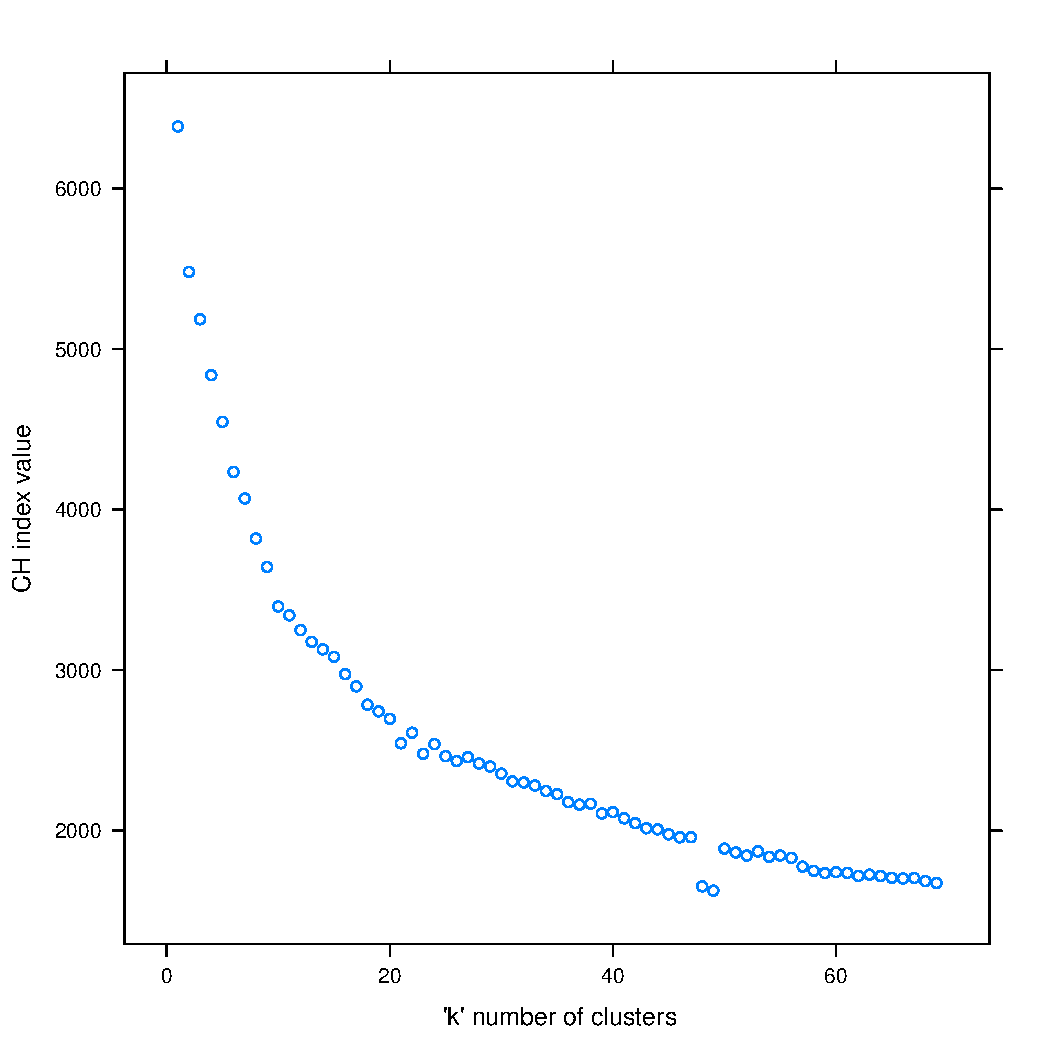
\includegraphics[width=0.5\textwidth]{figs/capitulo5/CHindex}
\caption{Calinski-Harabasz index by 'k' number of clusters}
\label{CHindex}
\end{figure}
 
\begin{equation}\label{eq:total_RMSE}
  RMSE_T = \frac{c-1}{k-1}RMSE_{left}+\frac{k-c}{k-1}RMSE_{right}
\end{equation}


\nomenclature[k]{$k$}{number of clusters.}
\nomenclature[c]{$c$}{number of clusters where the 2 fit-lines split.}
\nomenclature[CH]{$CH$}{Calinski-Harabasz validity index.}
\nomenclature[RMSET]{$RMSE_T$}{Total root mean square error}
\nomenclature[RMSEleft]{$RMSE_{left}$}{Root mean squared error of the left-side linear regression.}
\nomenclature[RMSErigth]{$RMSE_{right}$}{Root mean squared error of the right-side linear regression.}

Where \textit{c} is the number of clusters where the graph is split into the two fit-lines, \textit{k} is the total number of clusters. The ``total root mean square error'' is a weighted error with two terms, one for each side of c in the graph. Each side has a heavier weight depending on the points involved in the fitting. The minimum of $RMSE_{T}$ gives us the optimum number of clusters of the data \citep{Zagouras2013} which are used in the following steps.
 
\end{itemize}
 
\subsubsection{Photovoltaic energy yield}

The simulation of a photovoltaic energy system is described in a previous chapter. Here it is summarized in order to do not miss the coherence of the text.\\

The assessment of the power output of a photovoltaic system is carried out in two main steps:

\begin{enumerate}

\item In first place, global irradiation on the horizontal plane $G(0)$, which is the most common variable obtained from data sources, has to be transformed into the plane-of-array irradiation,  $G(\alpha, \beta)$, where $\alpha$ is the azimuth angle and $\beta$ the inclination angle of the generator plane. Due to optical losses (reflection, angle of incidence, and dust), the irradiation available is reduced for the photovoltaic cells inside the panels and the plane-of-array irradiation is then denoted as effective irradiation on the PV generator $G_{eff}(\alpha, \beta)$.\\
Three different types of tracking types are considered for the photovoltaic generator that influences on the tilt of the panels:
\begin{itemize}
\item \textbf{Fixed} panels with an optimum angle of inclination that depends on the latitude of the place.
\item \textbf{North-South} oriented panels that track the sun daily varying the azimuth angle, we will refer to them as ``one axis''
\item \textbf{Two-axes} tracking system that allows variation of the azimuth and inclination angles, we will refer to them as ``two axes''.
\end{itemize}
  
\item Once the effective irradiation that reach solar cells has been assessed, second step is the transformation into power output that depends on the photovoltaic system. The photovoltaic system is composed of a PV generator, consisting of several PV modules, and an inverter to transform the DC current output from the generator into AC current to be integrated into the network. In order to estimate  potential for photovoltaic production, the term \textit{yield} is defined as the system energy produced divided by the power installed $[\si{\kilo\watthour\per\kilo\wattpeak}]$.

\end{enumerate}

%The detailed description of the transformation from global irradiation in the horizontal plane to global effective irradiation, as well as the methods to assess power output from the PV generator are in the appendix A.

\subsubsection{Variability and complementarity}

The metric to analyze interannual variability is the coefficient of variation, CV Eq.\ref{eq:CV}, which is defined as:

\begin{equation}\label{eq:CV}
  CV=\frac{\sigma}{\overline{X}}
\end{equation}

In this equation, $\sigma$ is the standard deviation of the variable analyzed and it is divided by the mean of the variable in the period of the study. Sometimes CV is represented in percentage. This measure is dimensionless and can be applied in different time scales, which is helpful for comparisons.\\

To assess complementarity of the solar resource in the area of study, the Pearson's correlation coefficient between the time series of pairs of clusters Eq.\ref{eq:pearson} is calculated:

\begin{equation}\label{eq:pearson}
  \rho_{i,j}=\frac{\sigma_{c_i,c_j}}{\sigma_{c_i}\sigma_{c_j}}
\end{equation}

In this equation, $c_i$ and $c_j$ are the time series corresponding to the clusters $i$ and $j$. The concept of complementarity is associated with negative correlations between sub-regions of a wider area. If there is such a complementarity, a positive change in the variable for one of the clusters will be associated to a negative change for the other one. This is relevant for identifying spatial compensation possibilities and reducing overall variability in a network with high penetration of solar PV energy.\\

Complementarity can occur in different scales, either spatial or temporal and to understand it sometimes is a matter of balance. Spatial resolution for the complementarity assessment must be high enough to make sense of the comparison between zones, due to the fact that it is clear that geographically dispersed areas, far from each other, will have very different evolution of atmospheric variables, but may not be interesting from the electricity generation point of view. On the other hand, if the area of study is too small, atmospheric variables and therefore renewable resources will evolve in a very similar way. For such small areas, local complementarity between different resources can be analyzed, but not spatial complementarity of one resource. The methodology presented here addresses this issue by applying the inter-cluster comparison, that ensures homogenity within each cluster and differences between them.\\

Correlation coefficient for a long time series may hide changes in complementarity for shorter sub-periods with higher frquency correlations. For that reason a moving window is applied to the time series calculating the correlation coefficient and providing an indication of how complementarity between clusters varies during the whole period. Width of the window depends on the length of the time-series analysed.\\

In order to obtain the more important cluster pairs regarding complementarity, the median of the correlation coefficient series is calculated for each pair. After that, the cluster pairs are reordered from lower to higher values of this median correlation.\\
%, and the first 15 pairs (with the lowest median correlation) are selected as the most representative of complementarity, altought this number is rather arbitrary and also depend on the length of the time-series analysed.
 

\subsection{Results}

The optimal partition after having applied the clustering method is represented in figure \ref{clusters}. The CH validation procedure gives an optimum number of 19 clusters for the area, where each of the clusters has an homogeneous time evolution of solar irradiation. Due to the nature of clustering techniques, there is not an unique/best method to select the optimum partition. Another index (Davies-Boudin, \cite{davies1979cluster}) has been applied for comparison, and the obtained optimum number of clusters was of the same order than for CH index.
 
\begin{figure}[h!]
\centering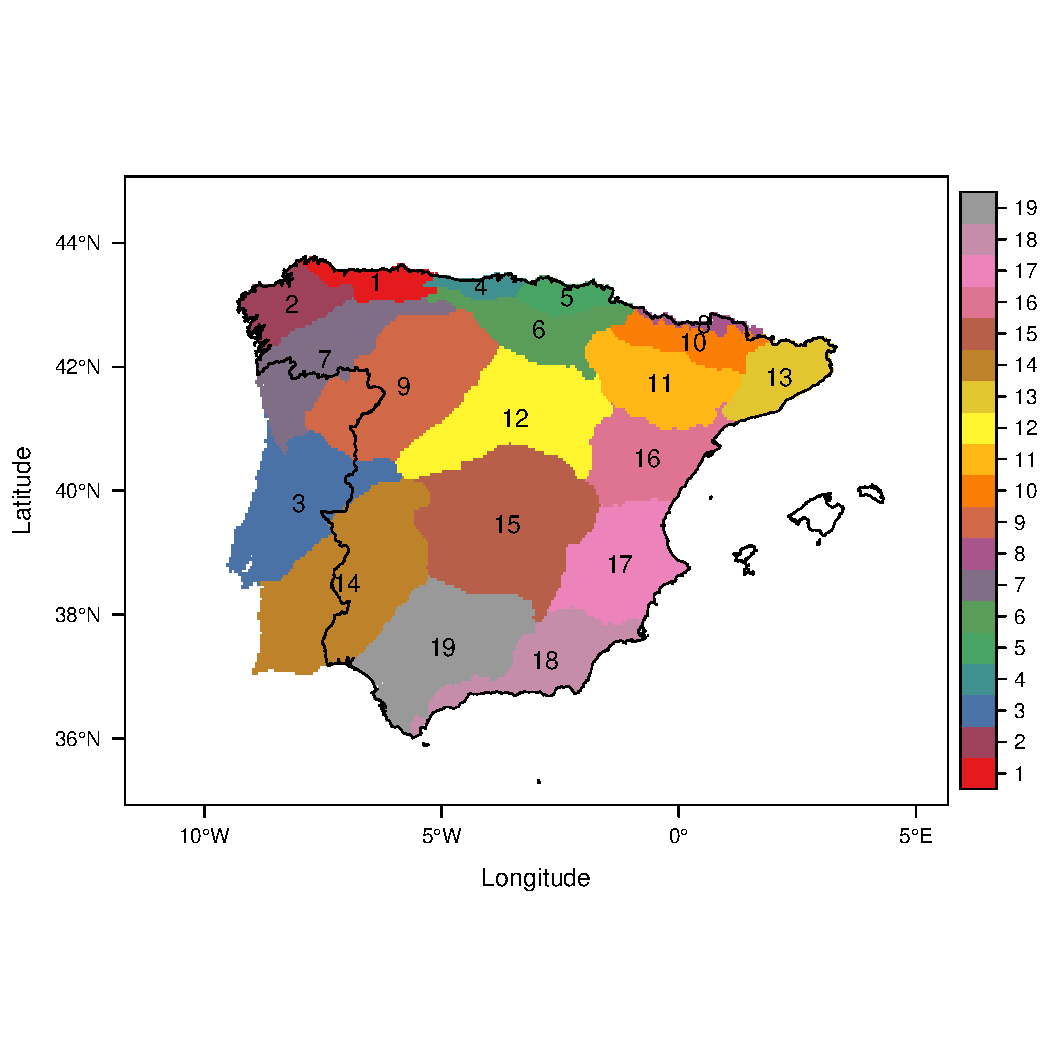
\includegraphics[width=0.6\textwidth]{figs/capitulo5/clusters2}
\caption{Optimal partition of 19 Clusters after applied the algorithm and the validity index}
\label{clusters}
\end{figure}

\subsubsection{Variability and complementarity results}

After regionalization, it is performed an analysis of solar irradiation on the horizontal plane and PV yield by tracking system, including their temporal variability.\\

Regarding interannual variability, we have calculated the CV of two time-aggregated means of solar irradiation and PV yield:

\begin{itemize}
\item On one hand it is applied for the yearly mean of daily irradiation $G_{d,y}(0)$ and yearly PV yield. This metric gives the variation of the of energy from one year to another and if it is low, general stability of the solar resource and PV production is guaranteed. 
\item On the other hand the interannual variability of the monthly time series $G_{d,m}(0)$ and monthly energy yield is also investigated in order to quantify differences in the annual cycle. 
\end{itemize}

The CV is also aggregated by cluster, in order to facilitate the intercomparison among areas.\\

%The general results about yield and variability can be found in the appendix. Here we present particularly relevant results that show the importance of considering different types of tracking methods, which is a fundamental aspect of the proposed scheme.\\

Power from the PV generator depends quasi-linearly with solar irradiation at the plane-of-array ($G_{eff}(\alpha,\beta)$), besides second order effects (spectrum, wind, etc) \citep{Perpinan2007} . Due to that the fixed typology is the one with lower yield because the amount of irradiation reaching cells is lower than the amount of energy reaching panels when trackers have one or two axes movements.

For areas where solar irradiation is higher, yield differences between trackers are higher. This can be seen in figure \ref{yearly_productivity_byCluster} where yearly mean yield for the 30-years period is aggregated by cluster and tracking system, and clusters are sorted vertically from less to more energy yield. A noteworthy result is that yield increase from fixed panels to one-axis panels is non-linear. This increase ranges between $17\%$ for the clusters with less solar irradiation, located at the northern coast (clusters 4, 5), and $30\%$ for the southern clusters with more solar irradiation (clusters 18, 19). In contrast, enegy yield increase from one-axis to two-axes panels is almost constant, around $12\%$ for all clusters. A consequence of the non-linear PV yield increase from fixed to one-axis panels is that the energy yield differences between clusters are much higher for tracking than for fixed systems. While for fixed panels PV energy yield varies between 1000 and 1450 $[\si{\kilo\watthour\over\kilo\wattpeak}]$, for two-axes systems it varies between 1350 and 2100 $[\si{\kilo\watthour\over\kilo\wattpeak}]$. These average values are coherent with results obtained in \cite{Antonanzas-Torres2013} when considering a value of 0.75 for the system performance ratio.
 
\begin{figure}[!tbp] 
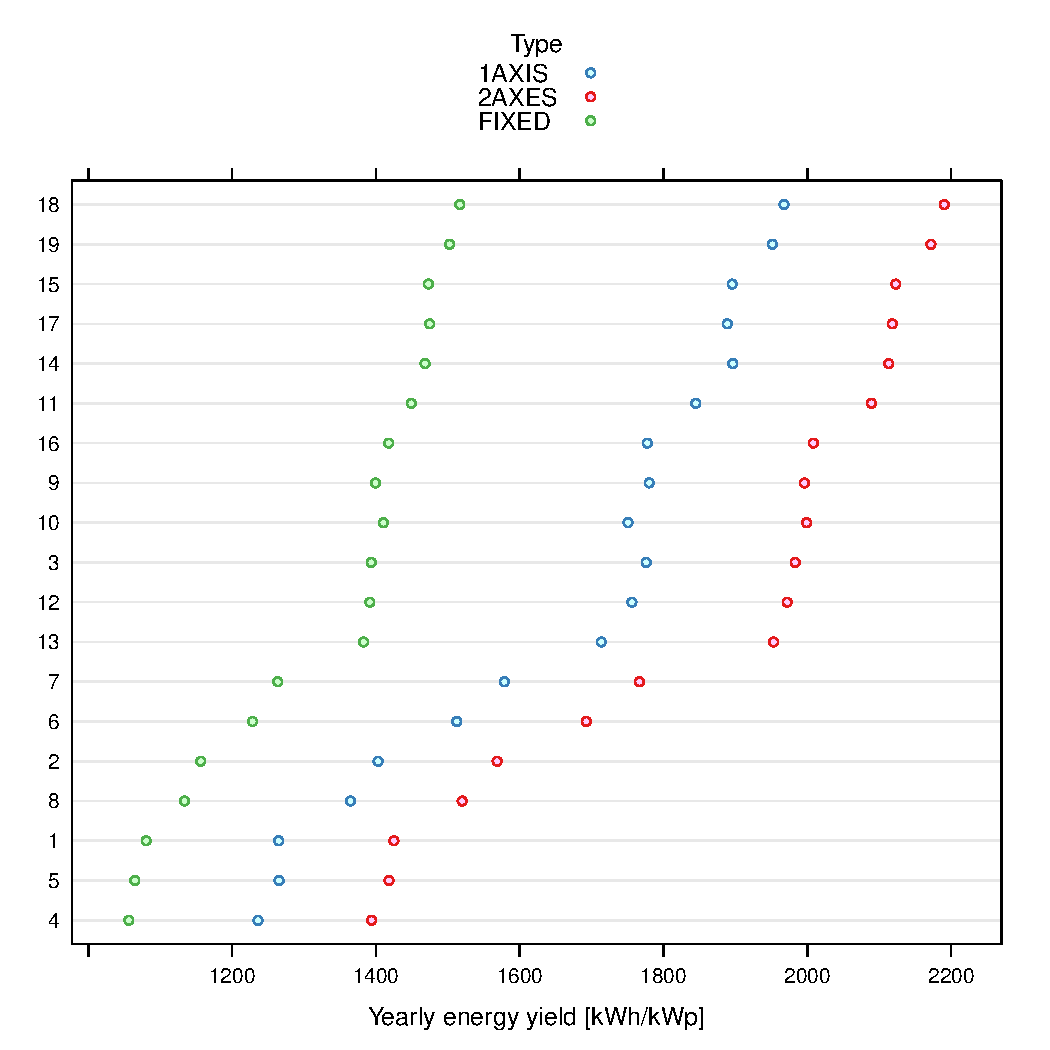
\includegraphics[width=0.6\textwidth]{figs/capitulo5/productividadTemp_byCluster.pdf}
\caption{Yearly mean of PV yield by cluster and for each tracking system $[\si{\kilo\watthour\over\kilo\wattpeak}]$. Values are sort from lower to higher yield values.}
\label{yearly_productivity_byCluster}
\end{figure}

Electricity price variations significantly depend on the variations of the monthly renewable electricity production from year to year. This time-scale is also the most influenced by the large scale circulation modes for solar potential in the Iberian Peninsula \citep{Jerez2013a}. The winter half of the year, from October to March, is especially variable.

The interannual variability for monthly yield is higher than for the irradiation at the horizontal plane, as it occurred for yearly values which results are in the appendix. In winter months, these differences in CV are much higher than in summer. This behavior is more pronounced in northern areas.

In order to quantify these differences in variability between solar irradiation and solar power output, the ratio between variability of yield by tracking system and solar irradiation is represented in figure \ref{ratiosCV} for each month and cluster. If CV of energy yield is higher than CV of solar irradiation, values are above one. On the other side values will be below one if CV of solar irradiation is higher than CV of energy yield. 

\begin{figure}
  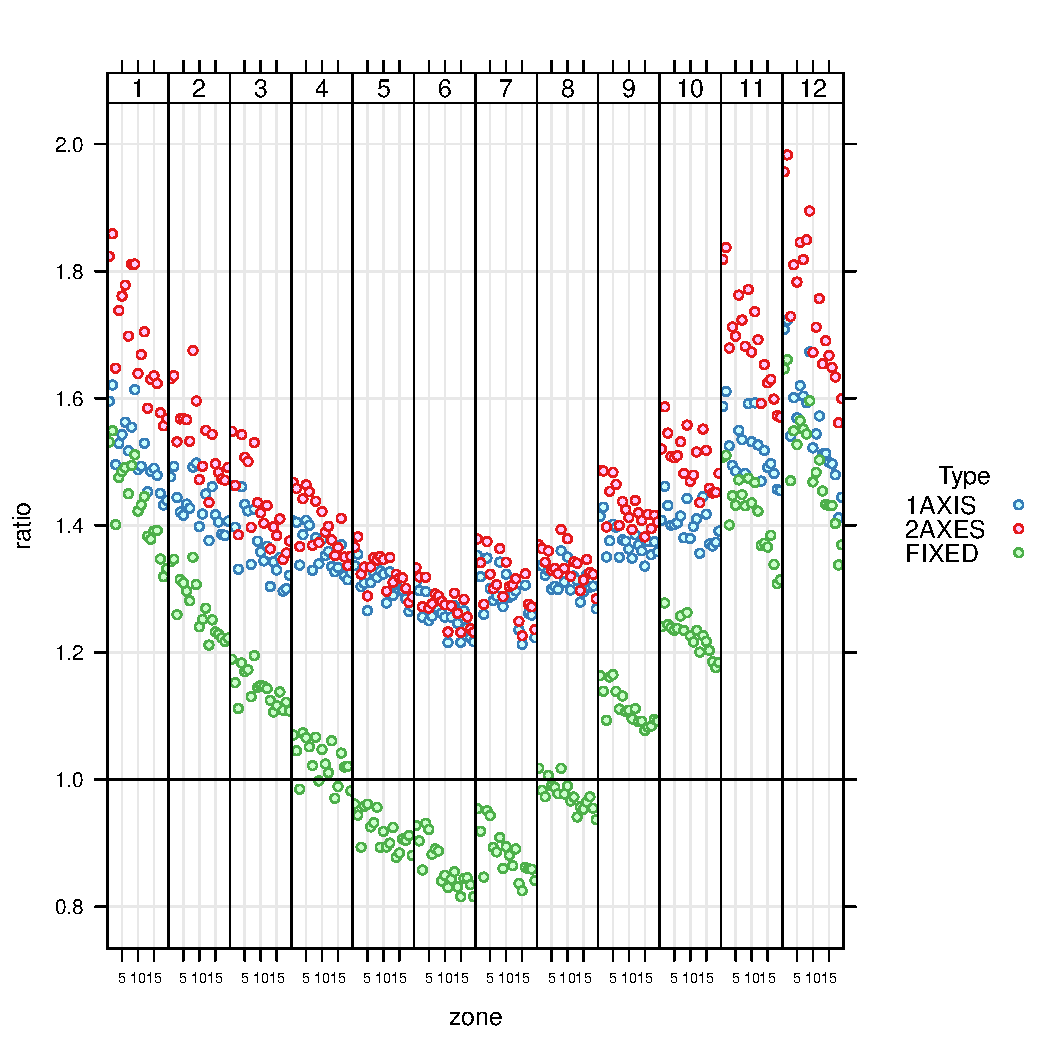
\includegraphics[width=0.6\textwidth]{figs/capitulo5/dotplot_ratio_zone.pdf}
  \caption{CV ratios between each type of tracking system and solar irradiation at the horizontal plane, grouped together by month in the graph. Ratios are calculated for each cluster, represented in the x axis. ``Fixed'' represents $\frac{CV_{fixed}}{CV_{G0}}$, ``1 axis'' is $\frac{CV_{1axis}}{CV_{G0}}$ and ``2 axis'' is $\frac{CV_{2axes}}{CV_{G0}}$}
  \label{ratiosCV}
\end{figure}

The highest ratios are obtained between $CV_{2axes}$ and $CV_{G0}$. The ratio of $CV_{1axis}$ is clearly lower in winter months, but is very similar in summer to the ratio of $CV_{2axes}$. Yield with an 'horizontal' axis tracker and 'two-axes' trackers increase the variability between $20\%$ in summer and more than $80\%$ in some areas in winter. The fixed typology ratio, $CV_{fixed}/CV_{G0}$ has a much wider range in the whole year. In winter months, it has values between 1.2 and 1.6, depending on the cluster, and is not far from the other two typologies. In contrast, this ratio decreases rapidly in summer months, reaching values below one between May and August. This means that for that period, variability of the 'fixed yield' is smaller than variability of solar irradiation at the horizontal plane.

The results of CV show that variability of PV energy yield at tilt panels is higher than variability of solar resource at horizontal plane in most cases, explained by the nature of solar irradiation at tilt panels and its dependency of solar irradiation at horizontal plane, \cite{Perpinan2009}.

The monthly time series are also selected for the complementarity analysis.

Regarding solar power complementarity, opposite-evolving time-series for different areas would strongly increase the reliability of the whole electric system, as shortfalls of solar irradiation in certain areas could be compensated by above-normal irradiation in others. However, this ideal situation is difficult to find in a rather limited area like the IP, at least for monthly timescales over a long time period of 30 years. In this case, the absence of correlation becomes also important, as it avoids simultaneous shortfalls or simultaneous above-normal values, and therefore softens the overall power production. The correlation matrix for the 30-year period and each month is in the appendix, showing the results for the whole period. In most cases, the correlation coefficient is highly positive, specially between pairs in the northern part of the Iberian Peninsula. For the southern part, the correlation coefficient is also positive but it decreases in July and August. There are some exceptions between the northern clusters 4 and 5 and the southern clusters 14 to 19, these pairs are only slightly correlated, not correlated or even slightly anticorrelated for some months.

Overall, southern and eastern clusters are uncorrelated at least during part of the year with northern and northwestern clusters. In some cases, the absence of correlation is found between nearby clusters: in winter months, the north-eastern cluster 11 (central Ebro valley) is uncorrelated to the closely-lying clusters 4, 5 and 8 (in the northern coast and Pyrenees). This is probably related to persistent atmospheric situations with north to northwesterly winds, that cause cloudiness in the windward clusters and clear skies in the leeward Ebro cluster, due to a foehn effect. This result points out the selective character of the clustering method.

It could be that the obtained clusters present higher complementarity in shorter sub-periods. We have divided the whole 30-year period in sub-periods of consecutive 15 years. The correlation coefficients have been calculated again for the resulting 15-year moving window, for each pair of clusters and for each month. In this way, we obtain how each correlation coefficient evolves during the 30 year period. The analysis has been applied for the four variables in the study: solar irradiation at the horizontal plane and PV energy yield for each tracking system.

The median value of the correlation coefficient series is calculated for each pair. Each serie comprises 12 monthly values for each of the 15-year moving windows. After that, the cluster pairs are reordered from lower to higher values of this median correlation, and the first 15 pairs (with the lowest median correlation) are selected as the most representative of complementarity. These cluster pairs are represented in figure\ref{horizonplot_rad}, showing the time-evolution of its correlation coefficient. These results are for solar irradiation on the horizontal plane. The corresponding figures for PV yield by tracking system are not shown due to the similar results obtained for this analysis.

\begin{figure}[h!]
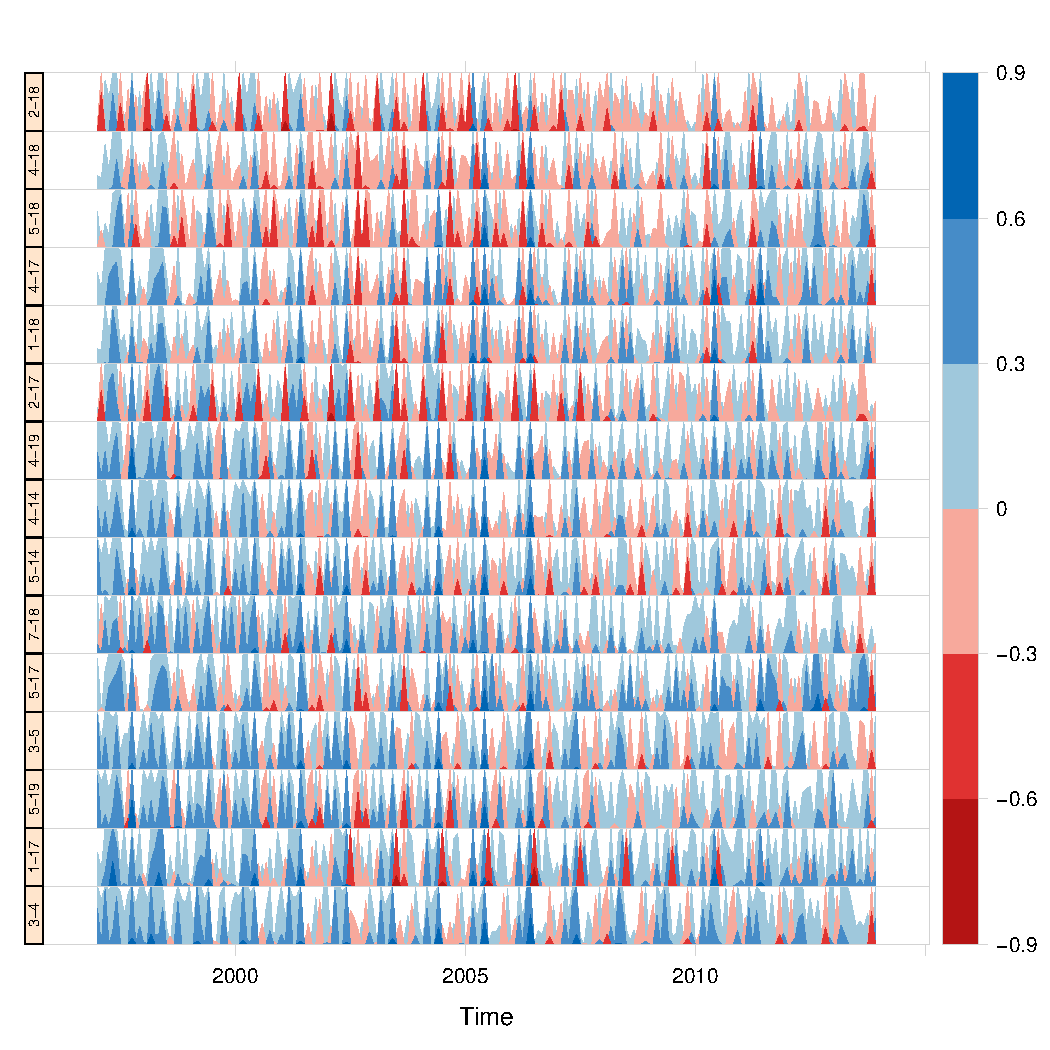
\includegraphics[scale=0.6]{figs/capitulo5/horizonplot_series_rad2}
\caption{Correlation coefficient of solar irradiation at the horizontal plane: evolution of a 15-year moving window of monthly values, for the 15 cluster pairs showing the smallest median correlation values. Monthly negative correlations (in red) and monthly positive correlations (in blue) are represented in the same axis to facilitate the comparison of the multiple time-series. Also, higher correlation values overlap with lower ones, enabling a compact presentation of all the information in a narrower plot. The cluster pairs are indicated on the left, while the year in the x-axis indicates the end of each 15-year moving window.}
\label{horizonplot_rad}
\end{figure}

The most relevant pairs in terms of complementarity include a northern (1, 2, 4 or 5) and a south-eastern cluster (17 or 18), as can be seen in figure \ref{horizonplot_rad}. The negative correlations for these pairs reach values below -0.6, at least in some 15-year sub-periods. These clusters are negatively correlated in most cases. Clusters 19 and 14 (southern and south-western IP) are also negative correlated with clusters in the north, although with lower values than the south-eastern clusters.

It is important to notice the appearance of cluster pairs 3-4 and 3-5 in this figure. These clusters are closer than the previously commented cases, which highlights the adequacy of the clustering method. All three are Atlantic coast clusters, but while cluster 3 includes part of the western coast, clusters 4 and 5 are northern coast areas. This fact, together with the position of the main mountain ranges, can explain their partially complementary behaviour.

%It is important to notice the appearance of cluster pairs 3-4 and 3-5 in this figure. These clusters are closer than the previously commented cases.  All three are Atlantic coast clusters, but while cluster 3 includes part of the western coast, clusters 4 and 5 are northern coast areas. This fact, together with the position of the main mountain ranges, can explain their partially complementary behavior. On the other hand, the 15-year moving window reveals interesting changes with time for all the cluster pairs, as there are higher and more frequent negative correlations in the middle 15-year sub-periods (those ending around 2005). 

In order to highlight the months with maximum anti-correlation,  figure \ref{horizonplot_months_rad} presents, for the same 15 cluster pairs as above, the minimum values of the monthly correlation coefficient (where the minimum for each month is calculated over all 15-year sub-periods). Differences between months are clearly observed in this graph. Only two months (March and June) show consistently positive values of this parameter, and therefore a low complementarity. In the other months, this parameter has predominantly negative values, revealing a certain degree of complementarity. July, August and September show rather low values and relatively high complementarity, which is important as these are months with a high productivity and also include the summer demand peak. In general,  for the second half of the year, the values of this minimum correlation value are lower than for the first half of the year.

\begin{figure}[h!]
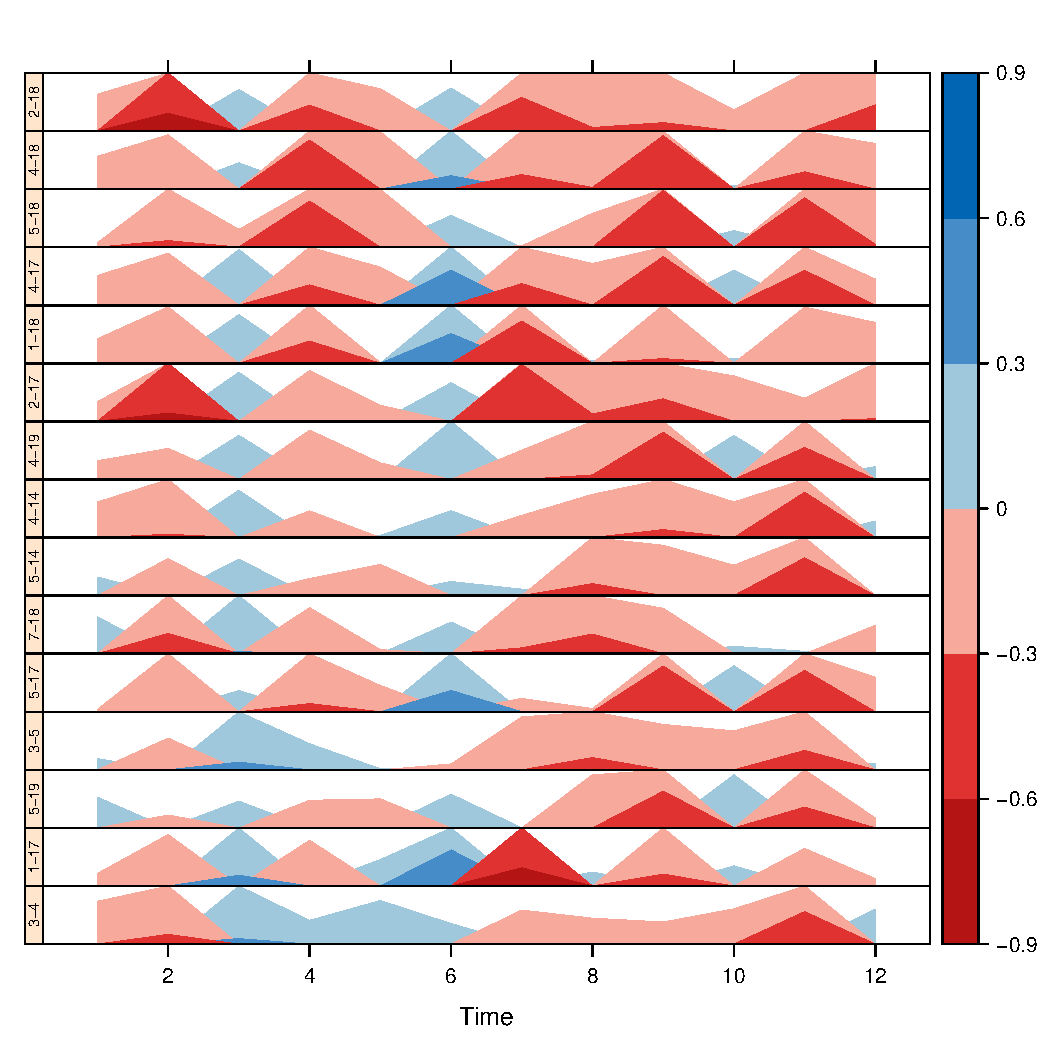
\includegraphics[scale=0.6]{figs/capitulo5/horizonplot_months_rad2}
\caption{Correlation coefficient of solar irradiation at the horizontal plane: minimum values of the monthly correlation coefficient, for the same cluster pairs as figure \ref{horizonplot_rad}. The minimum is calculated over all 15-year sub-periods. The type of representation of correlation values is the same as in figure \ref{horizonplot_rad}. The cluster pairs are indicated on the left, while the numbers in the x-axis indicate the months.}
\label{horizonplot_months_rad}
\end{figure}



\subsection{Conclusion}
\subsection{Summary}

\chapter{Impact of aerosols in photovoltaic energy production over the Euro-Mediterranean area}

\begin{abstract}

The increase in the photovoltaic energy installed capacity over the world leads to the need of a better understanding of solar resource and its variability. The aim of this work is to assess the influence of aerosols on photovoltaic energy production from seasonal to multi-decadal time scales. For this purpose we use various coupled aerosol-climate simulations that take into account the complex spatial and temporal patterns of natural and anthropogenic aerosols over the Euro-Mediterranean domain.

The results show that aerosols strongly influence the spatial pattern, seasonal cycle and long-term trend of PV production. The most affected area is Central Europe where sensitivity of PV production to aerosols is higher. The annual production loss due to aerosols ranges from no impact to $-16\%$ in The Netherlands, with variation depending on the area and on the typology of the tracking system. The summer production loss can even reach $-20\%$ over regions of Africa and Syria-Iraq.  

We conclude that aerosols can not be neglected in the assessment of PV production at large time scales over the Euro-Mediterranean area. Besides, the potential increase in energy due to reduction in the antrophogenic aerosols is shown in the simulation of the brightening period over Europe, with an increase of 2000 ${\kilo\watthour\over\kilo\wattpeak}$ in a PV lifetime for the most affected areas. It illustrates the evolution that PV potential could follow in highly polluted areas through the effective implementation of pollution control measures.  
  
   
\end{abstract}
 
\begin{keyword}
\texttt{Photovoltaic production variability\sep Aerosols\sep Regional Climate Modeling}
\end{keyword}

\end{frontmatter}

\linenumbers

\section{Introduction}


In the last decades there has been an overall increase in the deployment of photovoltaic (PV) power plants over the world, demanding research in the fields that contribute to a better integration of this technology into the electricity system. Due to the variability of solar resource, a comprehensive study of its spatiotemporal behavior is needed.

Aerosols particles influence the climate system directly, affecting the Earth’s radiation budget by scattering or absorption of solar radiation, or indirectly, changing cloud properties. Due to their importance in the amount of solar radiation that reaches the Earth’s surface and their effect in the changing climate, the evaluation of their impact on the solar resource for energy purposes is of special interest.

A general lack of well-spread surface stations, which provide solar radiation measurements, has made the satellite information the main and most reliable source of data up to now, due to its spatial and time resolution \citep{Posselt2012, Ineichen2014}. However, satellite retrievals were not available several decades ago and they do not allow to quantify the effect of specific factors on solar irradiance. Thus for investigating long-term statistics and to disentangle the various factors influencing solar resource, a different approach is needed. Models are the best tool to understand processes that occur in the atmosphere and their link with the resource variability, as individual factors can be included or removed in them, allowing the isolation of their effects.

Due to the increasing concern about the availability of renewable energy resources under climate change scenarios, climate modeling has revealed itself as a valuable tool for evaluating future energy potential \citep{Crook2011, Gaetani2014, Gaetani2015, Jerez2015, Jerez2015climix, Tobin2016}. However, representation of the clouds is still one of the main challenges for these models, and the spatio-temporal variability of aerosols is rarely taken into account in some of regional climate models \citep{Bartok2017}, which could lead to significant errors in PV power forecasting or future energy estimations \citep{Rieger2017}. Such climate simulations have to be combined with an accurate PV model capable of reproducing the system performance. Existing studies analysing the influence of aerosols on solar irradiation lack spatial detail (because of the use of relatively coarse global climate models) and/or do not apply a detailed PV production model \citep{Bergin2017}. 

The Mediterranean region is considered as highly influenced by aerosols coming from different sources \citep{Lelieveld}. These aerosols have a deep impact on the climate of the region \citep{Nabat2014, Nabat2014a}, thus on the shortwave solar radiation reaching the surface \citep{Mallet2016}. Regarding possible changes in antrophogenic aerosols in the future \citep{Gaetani2014, Jimenez-Guerrero2011}, the relevance of the near-term climate change scenarios and the expected PV deployment, the study of the Euro-Mediterranean area is important for solar energy.

In this work we use a regional climate model \citep{Nabat2014} with a realistic aerosol representation combined with an accurate PV model \citep{Lamigueiro2012}. The influence of these aerosols in the spatiotemporal variability of PV production over the region is quantified. The analysis is made in present climate conditions for simulations between 2003 and 2009 and different tracking types are considered in the study, due to the different sensitivity of each typology to changes in solar radiation \citep{Gutierrez2017}. On the other hand, the impact that trends in antrophogenic aerosols have in PV energy production is also investigated using longer simulations for the ``brightening'' \citep{Wild2005} period, 1980-2012, reflecting how pollution control policies could benefit the PV energy production in highly polluted areas.

This paper is organized as follows: in section 2 the climate and the photovoltaic model are described. In addition, there is a description of the aerosols and the datasets used for evaluation. Section 3 presents the results and shows the impact of aerosols on photovoltaic energy production. It is organized depending on the space-time scale analysed and there is a subsection for the tracking system sensitivity.  Flinally, section 5 is a discussion section for limitations and future perspectives and section 6 shows the main conclusions.

\section{Data and Methods}

Different climate simulations are used as an input of a PV power model. These climate simulations provide the daily-mean shortwave solar radiation, SSR, at the surface. The energy production model simulates the performance of a general photovoltaic system and includes different tracking types, considering the tilt of photovoltaic panels as a relevant component of the whole assessment. Computation of the photovoltaic energy model is made using the R open-source package named solaR \citep{Lamigueiro2012}.

\subsection{Climate Data}

The climate model used in this study (CNRM-RCSM4,\citep{Sevault2014}) is a coupled Regional Climate System Model (RCSM) dedicated to the study of the Mediterranean climate. CNRM-RCSM4 is one of the RCSMs contributing to the multi-model Med-CORDEX initiative \citep{Ruti2016}. It has the specificity to represent various components (atmosphere, land surface, river, ocean) of the Mediterranean regional climate system at high-resolution as well as their high-frequency coupling. The horizontal resolution is 50 km for the atmosphere, the land surface and the river network, and about 10 km for the Mediterranean Sea. In addition, the atmosphere part of the model, the so-called ALADIN-Climate version 5.2 \citep{Colin2010} is one of the few available Regional Climate Models which can take into account a realistic representation of the spatiotemporal variability of the aerosols \citep{Nabat2014}. The model has been extensively described, evaluated and intercompared with other Med-CORDEX models in previous studies, \cite{Sevault2014, Nabat2014, Nabat2014a,Flaounas2016, Gaertner2016, DellAquila2016, Harzallah2016, Cavicchia2016}

The detailed interannual aerosol dataset used in the climate simulations \citep{Nabat2013}, NAB13, is able to reproduce the spatiotemporal variability of AOD (aerosol optical depth) over the Mediterranean region. It improves the representation of aerosols against older climatologies commonly applied in regional climate studies like \cite{Tegen1997} or \cite{tanre1984first}.

The NAB13 dataset includes five different aerosol species: Sea Salt, Black Carbon, Sulfate, Organic Carbon and Desert Dust (ss, bc, su, or, sd); with spatial and temporal variability. It is based on a blending of a satellite-derived AOD product and a high-resolution regional climate model using up-to-date interactive aerosols module. This dataset has also been evaluated against ground stations \citep{Nabat2013}.

During the eighties, some policies against the emissions of certain types of antrophogenic aerosols were implemented in Europe, which has been linked with the observed increase in the shortwave solar radiation in the area \citep{Wild2005}. For simulations over this commonly named ``brightening period'' (1980-2012), a trend for sulfate aerosols is included in NAB13, being able to reproduce the shortwave solar radiation trend observed over Europe since 1980 \citep{Nabat2014a}.

There is a large spatial and seasonal variability of the AOD at 550nm over the Euro-Mediterranean. Spring and summer months are highly influenced by dust aerosols in the south of the domain. In winter, antrophogenic aerosols dominate in central Europe and during autumn, there are few areas with high values in opposition to the rest of the domain.

The domain considered in the simulations covers the Mediterranean area in addition to a large part of Europe (see figure \ref{fig:mapapral}).

For the first period, 2003-2009, a pair of runs is analysed. We refer to them as \textbf{AER} and \textbf{NO-AER}. The AER simulation includes the NAB13 dataset, whereas no aerosols are included in NO-AER. This pair allows to easily attribute the obtain differences to the aerosols effect, therefore to quantify the impact of aerosols on the Euro-Mediterranean SSR and PV productivity. It is an important point considering the fact that some of the state-of-art RCM do not include aerosols in their simulation, so it gives an idea of that missing forcing.

Secondly, a longer simulation between 1980 and 2012, \textbf{TREND}, covering the ``brightening'' period observed in Europe is also analysed. It will show the effect of a decreasing trend in sulfur aerosols on the shortwave solar radiation and on the PV productivity.  

A summary of the different simulations is reported in table \ref{tabSIM}.

\begin{table}
  \begin{tabular}{>{\raggedright}m{2cm}>{\raggedright}m{3cm}>{\raggedright}m{2cm}}
    \toprule 
    Simulation & Aerosols & \centering{Period}\tabularnewline
    \midrule
    AER & NAB13 & 2003-2009
    \tabularnewline
    \midrule
    NO-AER & Not included & 2003-2009
   \tabularnewline
   \midrule           
  TREND & NAB13 + sulfates trend & 1980-2012
   \tabularnewline
    \bottomrule
  \end{tabular}
  \caption{Simulations of the CNRM-RCSM4 regional climate model to obtain SSR and temperature as input of the photovoltaic model, period and representation of aerosols in each simulation.}
\label{tabSIM}
\end{table}

\begin{figure}[h!]
\centering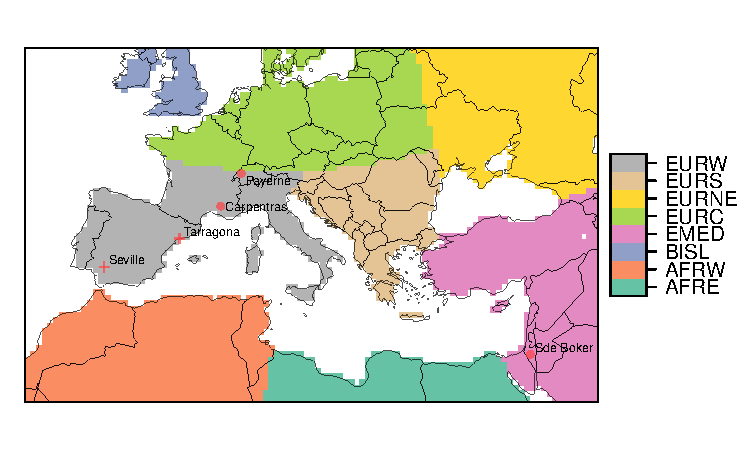
\includegraphics[width=0.7\textwidth]{figs/capitulo6/zonasPuntosLabel.pdf}
\caption{Areas defined to evaluate the difference in solar radiation between the satellite and the climate model simulations: Western Europe, EURW; Southern Europe, EURS; North-Eastern Europe, EURNE; Central Europe, EURC; Eastern Mediterranean, EMED; British Island, BISL; Western Africa, AFRW; Eastern Africa, AFRE. The location of the BSRN stations is represented with points ``.'' and the two PV plants are plotted with ``+'' in orange.}
\label{fig:mapapral}
\end{figure}

 
\subsection{PV model description}

In this section we make use of the commonly used terms: shortwave solar radiation, SSR, is equivalent to the global irradiation at the horizontal plane $G(0)$, which is composed of the beam component, $B(0)$, the diffuse irradiation, $D(0)$, and the albedo $R(0)$.

A photovoltaic energy system is mainly composed of the generator, consisting of several modules that include the cells to transform solar radiation into electricity, and the inverter, which transforms direct current into alternate current to be integrated into the electricity network. The assessment or estimation of the power output of a PV system implies modeling its components. For this purpose, two main steps have to be considered. The first is related to the amount of energy that reaches the generator surface and the other is based on the performance of the electrical components. The procedure is described in \cite{Perpinan2009} and the same methodology was applied in \cite{Gutierrez2017}.

1) Global irradiation at the horizontal plane $G(0)$, as an output of the climate model, has to be transformed into the global effective irradiation, $G_{eff}(\alpha, \beta)$, which is the amount of energy reaching the tilted surface of the generator (where $\alpha$ is the azimuth angle and $\beta$ the inclination angle) after considering reflection losses, angle of incidence and accumulated dust.  

First, for the decomposition of $G(0)$, empirical equations that correlates the \textit{clearness index} and the \textit{diffuse fraction} \citep{Page1961} are used. The clearness index is a measure for the energy lost when solar irradiation goes through the atmosphere, and the diffuse fraction is the relationship between the diffuse component, $D(0)$, and the global irradiation at the horizontal plane $G(0)$. Its value is the amount of the diffuse component in global irradiation.

The equations that relate the clearness index to the diffuse fraction depend on the place and time scale involved. There are many relationships proposed depending on the area of the study \citep{deMiguel2001, Gopinathan1995}. For daily time-scales, the equations that relate the clearness index and the diffuse fraction proposed by \cite{Aguiar1992} are used in our case. 

Three different tracking types are considered for the photovoltaic generator and the equations describing movements and relative position between the system and the sun are described in \cite{Perpinan2009}
\begin{enumerate}
\item \textbf{Fixed panels} with an optimum angle of inclination that depends on the latitude.
\item \textbf{One} axis trackers, with a generator rotating on an axis oriented North-South. We will refer to them as \textbf{“one”}.
\item \textbf{Two-axes} tracking system that allows variation of the azimuth and inclination angles, we will refer to them as \textbf{“two”}.
\end{enumerate}

To obtain irradiation components in the tilted surface at daily time scale, it is first necessary to estimate the irradiance profile using empirical relationships \citep{Collares-Pereira1979}. Irradiance profile is then transformed into its components at the tilted surface and integrated in time to obtain the energy reaching the generator surface. Direct irradiance can be transformed to the tilted surface using only geometrical criteria whereas the diffuse fraction is obtained with the model proposed by \cite{hay1985estimating}. This model considers an approximation where the sky sphere is seen by the generator as isotropic except for the circumsolar region, which is considered to emit direct irradiance. The albedo component is considered as isotropic, due to the fact that its contribution to global irradiance is low. 

Finally, we apply equations from \cite{Martin2001} to obtain $G_{eff}(\alpha, \beta)$. It includes optical losses due to the fact that, except for the two-axis tracking system, the incident irradiation deviates from the normal of the generator. Also, transmittance losses are included for accumulated dust over the surface, considering a ``moderate dust degree'' in the terms used in the referenced paper \cite{Martin2001}. In this case, any spatial distinction is considered and the same coefficient values are used to calculate angular and transmittance losses. 

2) The second step is the transformation into power output, depending on the electrical characteristics of the components in the photovoltaic system and second order effects like temperature. A summary of the modules and the inverter model can be found in table \ref{table1}. Detailed information about this step can be found in \cite{Perpinan2009}.

Ambient temperature is needed since the efficiency of the cells decreases with the increase of temperature, assuming a linear relationship. In this work we use the equation of \cite{Crook2011}, to calculate the daytime temperature from the daily maximum and minimum temperature, obtaining a daily profile. 

Computation of the photovoltaic energy model is carried out with the \texttt{solaR} package \citep{Lamigueiro2012}. This package implements in R a set of functions that include the sun apparent movement equations, the solar irradiation and irradiance decomposition, transposition models, and the PV generator and inverter models. 

\begin{table}[h!]
  \begin{tabular}{>{\raggedright}m{2cm}>{\raggedright}m{6cm}}
    \toprule 
    Element & Method\tabularnewline
    \midrule
    PV generator & Identical modules with
    $dV_{oc}/dT_{c}=0,475\frac{\%}{\celsius}$ and $NOCT=47\celsius$. 
    The MPP point calculated as in \cite{garcia2005caracterizacion}). \tabularnewline
    \midrule
    Inverter & Efficiency equation proposed in
    \cite{jantsch1992results}:  
    \begin{equation}
      \eta_{inv}=\frac{p_{o}}{p_{o}+k_{0}^{o}+k_{1}^{o}p_{o}+k_{2}^{o}p_{o}^{2}}
    \end{equation}
    where $p_{o}=P_{ac}/P_{inv}$ is the normalized output power of the inverter. The characteristic coefficients of the
    inverters are: $k_{0}^{o}=0.01$, $k_{1}^{o}=0.025$, $k_{2}^{o}=0.05$.\tabularnewline
    \midrule
    Other losses & \begin{itemize}
    \item Average tolerance of the set of modules, $3\%$.
    \item Module parameter dispersion losses, $2\%$.
    \item Joule losses due to the wiring, $1.5\%$.
    \item Average error of the MPP algorithm of the inverter, $1\%$.
    \item Losses due to the MV transformer, $1\%$.
    \item Losses due to stops of the system, $0.5\%$.
    \end{itemize}
    \tabularnewline
    \bottomrule
  \end{tabular}
  \caption{Calculation procedure for the estimation of energy produced by a PV system from daily global horizontal irradiation data. Left column represents the element of the PV system and the right column the equations and methods used in each case for the efficiency of the elements.}
  \label{table1}
\end{table}

\subsection{Datasets for evaluation}
\subsubsection{Satellite product: CM-SAF.}

CM-SAF (Climate Monitoring Satellite Application Facility) \citep{Schulz2009} was created as part of EUMETSAT Satellite Application Facility (SAF) when the importance of “contributing to the operational monitoring of the climate and the detection of global climatic changes” was recognized. Besides its operational products, they provide Climate Data Records generating long-term data, which is a valuable product for climate variability studies. In this work, the SARAH \citep{Muller2015} dataset for daily shortwave solar radiation, SSR, is used with an horizontal resolution of 0.44º to be consistent with the model simulations and for the period 2003 and 2009. For this product, the $85\%$ of absolute differences with shortwave solar radiation measurements is below 10 $\watt/m^2$ for monthly values and 13 $\watt/m^2$ for daily means.

Concerning aerosols representation, the satellite dataset includes information from MACC \citep{Benedetti2009, Morcrette2009}, provided by the European Centre for Medium-Range Weather Forecasts (ECMWF). Monthly long-term means of a 0.5x0.5 degrees grid are spatially interpolated to assign the values of each pixel.

\subsubsection{BSRN stations}

The BSRN (Baseline surface radiation network) \citep{Ohmura1998} is a set of ground-based measurements, from the WRCP Radiative Fluxes Working Group. It was created for supporting research in the radiation budget of the Earth-atmosphere and the radiation distribution, considering its main role in climate processes. The main objective is to provide high-quality measurements that are able to deal with the scarcity of the existing radiometric network. Although there are not many stations available for the period of the study in the Euro-Mediterranean domain, the high quality data provided by BSRN is necessary for a first evaluation of the climate simulations.

The three stations of the BSRN network used in this study (Payerne, Carpentras and Sede Boker) covered the period 2003-2009 and provide SSR monthly data. Their location is represented in figure \ref{fig:mapapral} together with the PV plants considered in the study.  

\subsubsection{Temperature data: ECAD}

The PV production assessment calculated using the SSR from satellite data needs also the temperature for the performance of cells inside the module. The gridded E-OBS data set from the EU-FP6 project ENSEMBLES \citep{Haylock2008} is used in the energy production model at daily resolution. Mean, maximum and minimum temperature from the dataset, in a spatial resolution of 0.25º, are interpolated to the same grid of the climate model. 

\subsubsection{PV production data}

Data from two different power plants are used for the evaluation of the simulated PV power and the assessment of the added value of the aerosol inclusion in the climate simulations.

The two power plants are in the Iberian Peninsula and their location represented in figure \ref{fig:mapapral}. The first one, located in Tarragona in the North-East area, is a PV system with fixed structure. The second one is a two-axis tracking PV plant located in Seville, in the South of Spain. Details of both PV power plants are in table \ref{tabPlants}, including the electrical characteristics of their components. 

\begin{table}[h!]
  \begin{tabular}{>{\raggedright}m{1.5cm}>{\raggedright}m{3cm}>{\raggedright}m{3cm}}
    \toprule 
     & \centering{Seville} & \centering{Tarragona}\tabularnewline
    \midrule
    Type & \centering{two-axes} & \centering{fixed} 
\tabularnewline
    \midrule
    Generator & \centering{$P_{g}=27.31$ $\kilo\wattpeak$}\\ 
                 \centering{$N_{mp}=12$}\\
                 \centering{$N_{ms}=11$} & \centering{$P_g=100.18$ $\kilo\wattpeak$}\\
                               \centering{$N_{mp}=27$}\\
                               \centering{$N_{ms}=35$}
   \tabularnewline
   \midrule
   Inverter & \centering{$P_{inv}=25$ $\kilo\watt$}\\
              \centering{$V_{min}=405$ $\volt$} & \centering{$P_{inv}=100$ $\kilo\wattpeak$}\\
                                \centering{$V_{min}=450$ $\volt$}
    \tabularnewline    
    \bottomrule
  \end{tabular}
  \caption{Summary of the electrical components of the two photovoltaic plants, including generator characteristics (generator power $P_g$, and modules in parallel and serie, Nmp and Nms) and the inverter characteristics (power of the inverter $P_{inv}$ and the voltage $V_{min}$).}
  \label{tabPlants}
\end{table}


Data of PV production are difficult to obtain due to confidentiality contracts. Moreover, when data are available time series are not always complete. Maintenance, modules substitutions, inverter problems and other stops in the production may lead to common time-gaps in the datasets. These limitations must be taken into account when establishing statistical comparisons between models and real data. In this case, the two PV power plants provide daily data within the period 2003-2009, the details are in table \ref{localData}. Monthly means of these data are compared against the monthly means of simulated daily PV productivity, energy produced by the power installed ${\kilo\watthour\over\kilo\wattpeak}$, with the models and the satellite. Only months with more than 15 days of data available are considered for the monthly mean and compared against simulated data.

\section{Results} 

Although the AOD dataset and the climate simulations used in this study have already been evaluated against observations and satellite datasets in \cite{Nabat2013, Nabat2014, Nabat2014a}, an additional assessment of the SSR form the climate simulations is also made in this work against the CM-SAF SARAH dataset \citep{Muller2015} for the period 2003-2009 and against some BSRN \citep{Ohmura1998} stations at a local scale. 
\subsection{Local scale}

Three different stations from BSRN cover the period between 2003-2009 with SSR monthly data. Stations are represented in figure \ref{fig:mapapral} with points. Also, two different power plants in Spain, represented in figure \ref{fig:mapapral} with a cross, are used to evaluate PV power simulations at a local scale. A summary of the data used in this section, the periods and the resolution can be found in table \ref{localData}.


\begin{table}[h!]
  \begin{tabular}{>{\raggedright}m{2cm}>{\raggedright}m{2cm}>{\raggedright}m{2cm}>{\raggedright}m{2cm}>{\raggedright}m{2cm}>{\raggedright}m{2cm}}
    \toprule 
    Data from & \centering{Seville} & \centering{Tarragona} & \centering{Payerne} &\centering{Sede Boker} &\centering{Carpentras}\tabularnewline
    \midrule
    Variable & \centering{PV productivity} & \centering{PV productivity} & \centering{SSR} & \centering{SSR} & \centering{SSR} 
\tabularnewline
    \midrule
    Time res. & \centering{day} & \centering{day} & \centering{month} & \centering{month} & \centering{month}
                    \tabularnewline
   \midrule
                                                                                            Period & \centering{518 {\small{daily values between:}} 02-07-2007\\30-11-2008} & \centering{300 {\small{daily values between:}} 01-01-2003\\19-03-2005} & \centering{2003-2009} & \centering{2003-2009} & \centering{2003-2009}
                  \tabularnewline    
 \midrule
    $\%$ no data & \centering{0} & \centering{8 $\%$} & \centering{0} & \centering{10.71 $\%$} & \centering{0}
                    \tabularnewline

 \bottomrule
  \end{tabular}
  \caption{Summary of the local data of PV power plants and SSR from BSRN stations used for the evaluation of the simulations. SSR is evaluated as input of the PV model and the PV output as the result of the whole modeling process.}
  \label{localData}
\end{table}

In figure \ref{fig:station} differences in monthly time series of SSR from simulations and satellite data and the stations measurements are represented.

\begin{figure}[h!]
  \centering\begin{subfigure}{0.4\textwidth}
    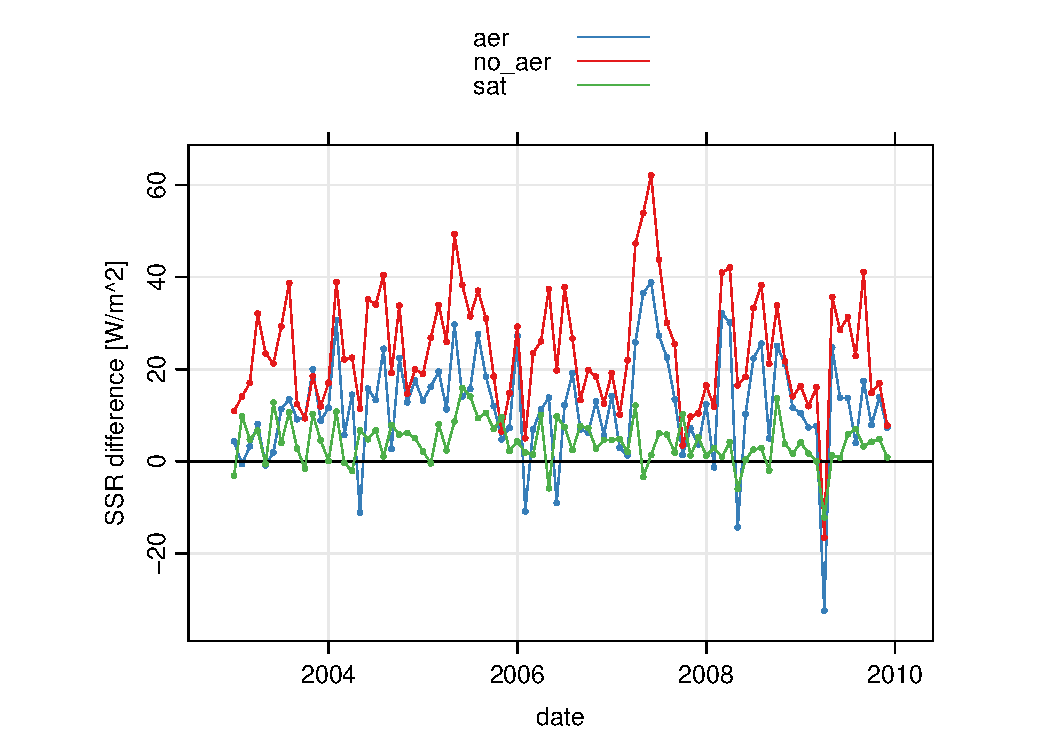
\includegraphics[width=1.2\textwidth]{figs/capitulo6/CarpentrasMesesDif.pdf}
    \caption{Carpentras}
    \label{Carpentras}
  \end{subfigure}
  %
  \centering\begin{subfigure}{0.4\textwidth}
    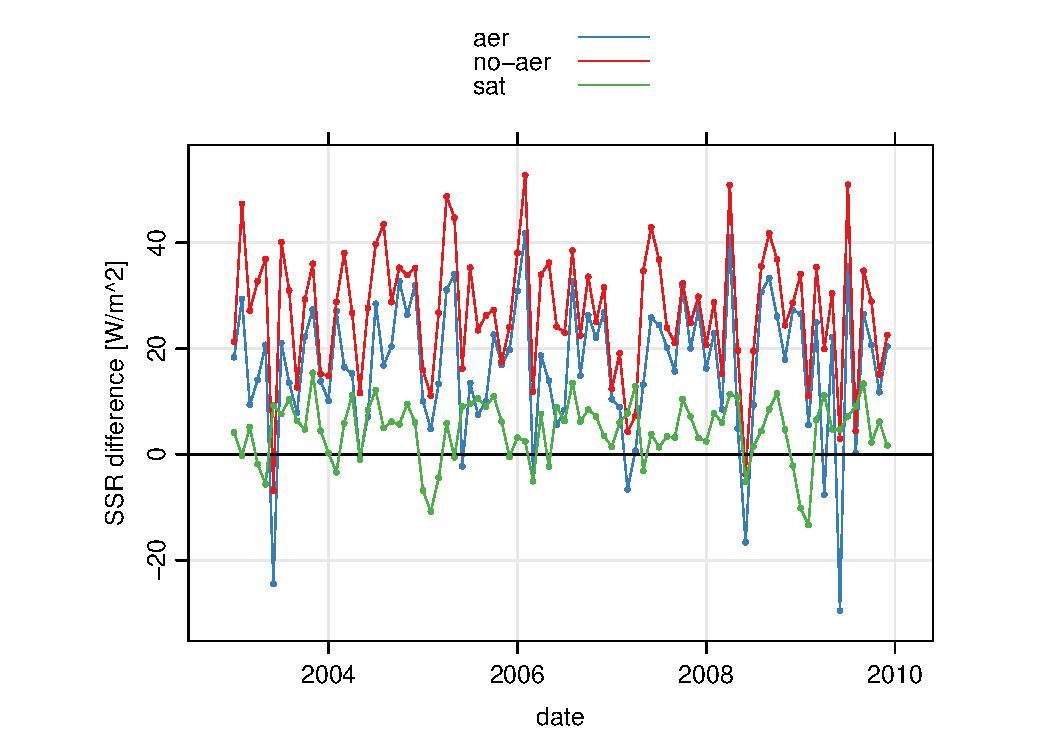
\includegraphics[width=1.2\textwidth]{figs/capitulo6/PayerneMesesDif.pdf}
    \caption{Payerne}
    \label{Payerne}
  \end{subfigure}
  %
    \centering\begin{subfigure}{0.4\textwidth}
    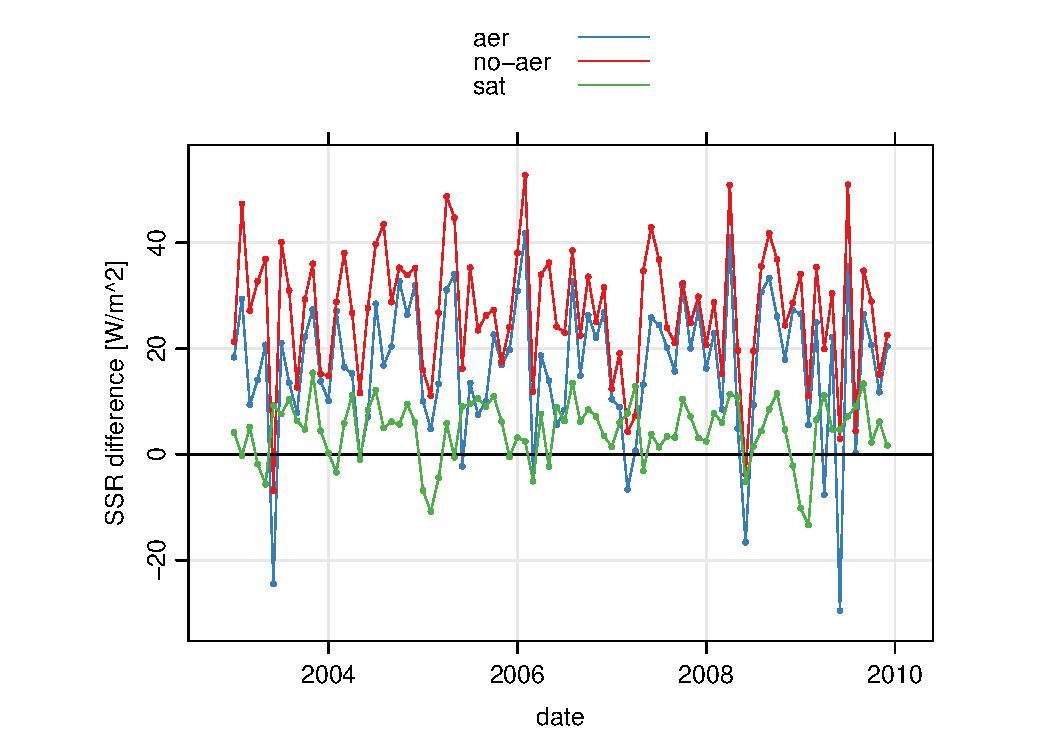
\includegraphics[width=1.2\textwidth]{figs/capitulo6/SedebokerMesesDif.pdf}
    \caption{Sede Boker}
    \label{fig:Sde Boker}
  \end{subfigure}
  \caption{Difference in SSR $\si{\watt\per\metro\squared}$ between both simulations and the satellite with respect to the data from BSRN stations (BSRN)}
    \label{fig:station}
\end{figure}

For the three stations, the satellite has better results than the simulations, although the error magnitude varies depending on the station. There is also a general improvement of the AER simulation against the NO-AER. Carpentras station is the one with lower bias with respect to the observed data \ref{Carpentras}. In the case of the Sede Boker station \ref{fig:Sde Boker}, there is a seasonal bias in the AER simulation. High negative differences appear from May to August, showing underestimation of the SSR in these months.

Several statistical measurements summarize the general performance of the SSR from the climate model and the PV simulations at each location and are reported in table \ref{RMSE_MAE_table}.

For the simulation of PV power output, the daily mean of PV production data averaged for each month is compared with simulated PV energy production at each power plant, using the three possibilities of SSR data as input: AER, NO-AER and SAT. For these simulations, in order to help with the visualization of the results a \textit{violin plot} is used to visualize the absolute error and its distribution.
For the Seville PV power plant, AER performs better than NO-AER and SAT simulations showing lower errors \ref{fig:figuraSEVILLA}. Besides, only AER has some negative errors, which means underestimation for some months, whereas the satellite and the NO-AER have only positive error values.

The median error for the AER simulation is less than 0.25 $\si{\kilo\watthour\per\kilo\wattpeak}$. Differences are concentrated around this value, which makes the distribution peaks around it in a narrow shape, although the range is wider due to higher values above 0.5 $\si{\kilo\watthour\per\kilo\wattpeak}$ that spread the distribution.

NO-AER simulation has a wider range of errors than AER and SAT, and a wider distribution. The satellite presents a median error close to 0.5 $\si{\kilo\watthour\per\kilo\wattpeak}$, as it could be expected from the evaluation and report of the CM-SAF dataset.

\begin{figure}[h!]
  \centering\begin{subfigure}{0.45\textwidth}
    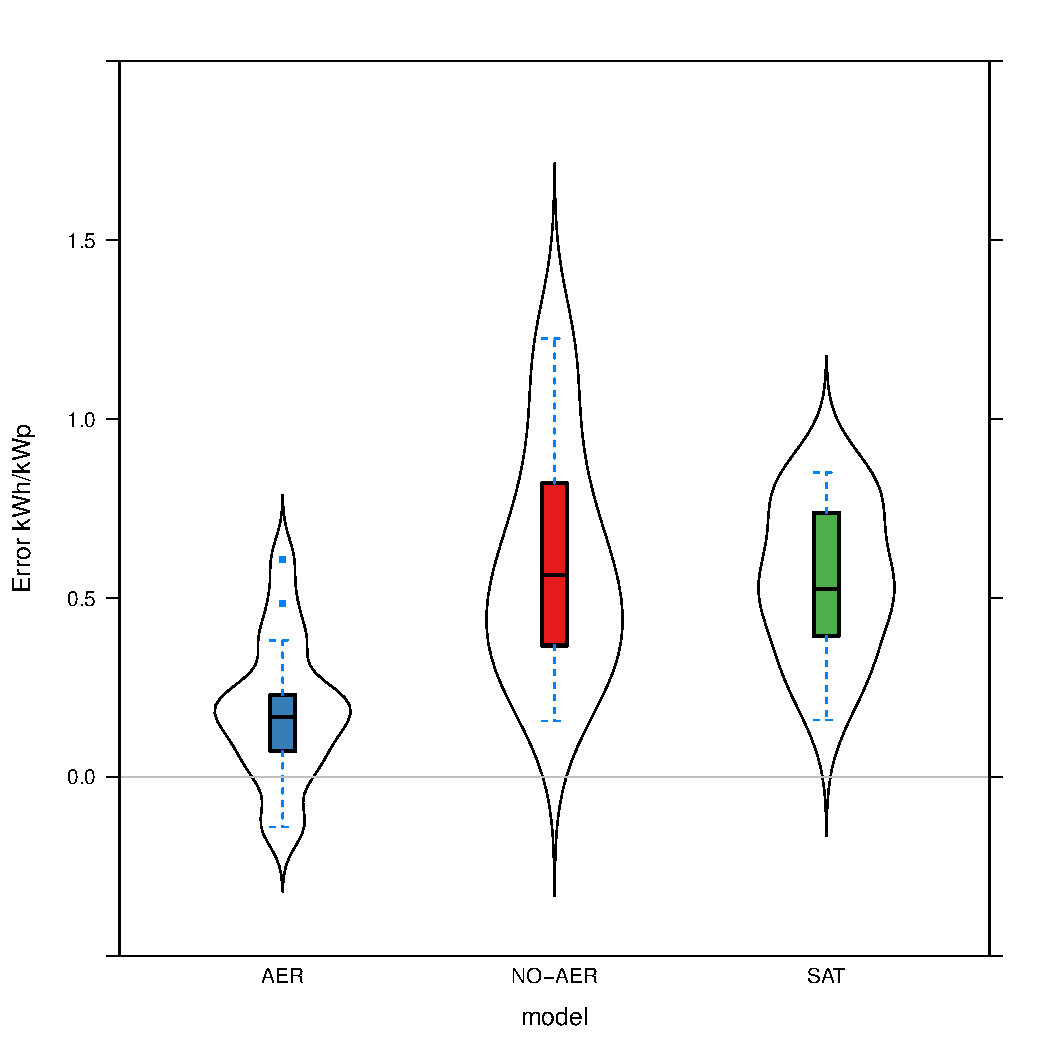
\includegraphics[width=1\textwidth]{figs/capitulo6/violinplorSeville.pdf}
    \caption{Seville}
    \label{fig:figuraSEVILLA}
  \end{subfigure}
  %
  \centering\begin{subfigure}{0.45\textwidth}
    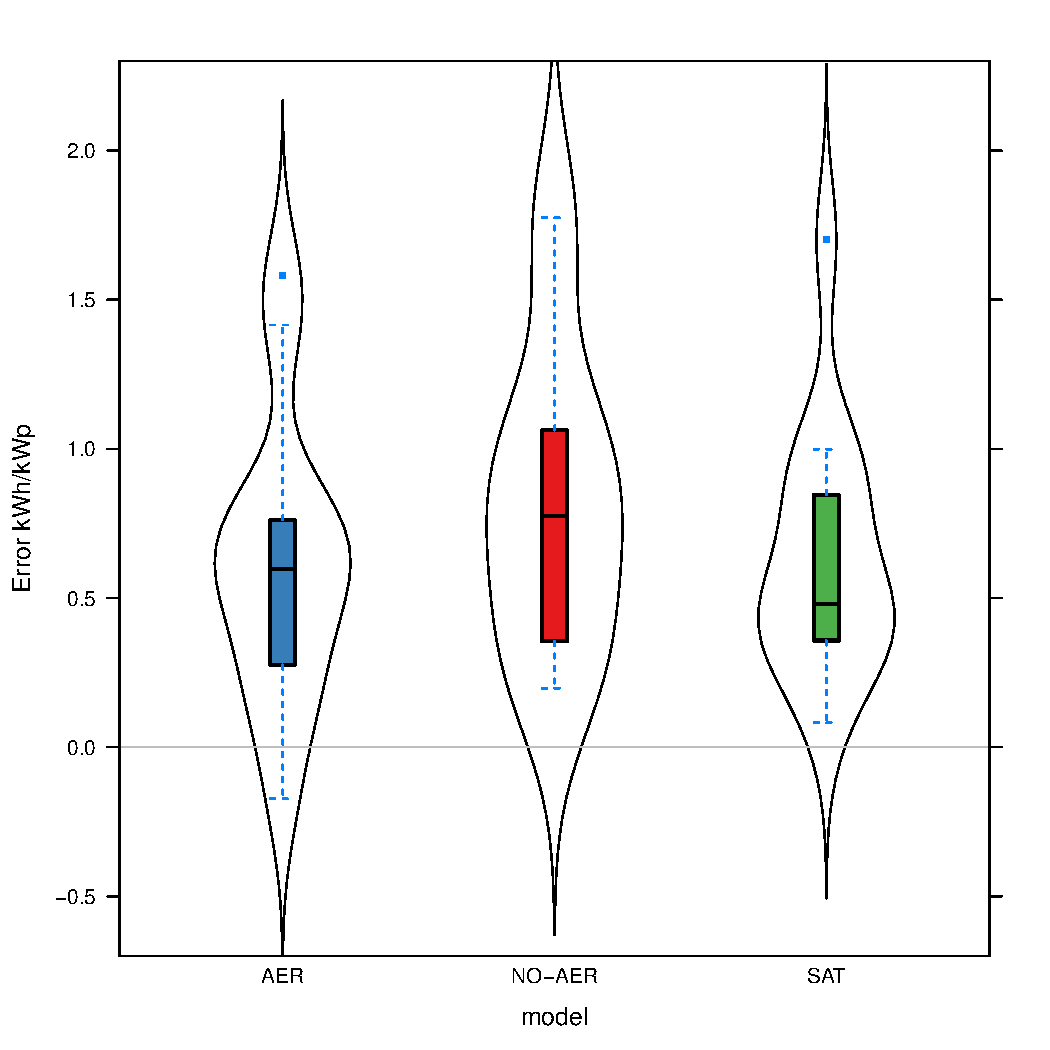
\includegraphics[width=1\textwidth]{figs/capitulo6/violinplotTarragona.pdf}
    \caption{Tarragona}
    \label{fig:violinTarragona}
  \end{subfigure}
  \caption{Distribution of differences in monthly mean of daily PV productivity $\si{\kilo\watthour\per\kilo\wattpeak}$ from Seville and Tarragona power plants and the simulated with the model, AER (blue) and NO-AER (red), and the satellite (green) in the same location. The period for Seville is from July 2007 to November 2008 and for Tarragona power plant from January 2003 to December 2005. The violin plot represents at the y-axis the probability density function of the variable, estimated with a kernel density estimation. Along this axis, the plot represents the shape of the variable distribution and it is duplicated by symmetry over an imaginary vertical axis to facilitate visualization. In this way it is easier to see not only statistical parameters represented in the boxplot, that it is also shown inside the violin, but also how the errors are distributed.}
    \label{violin}
  \end{figure}

\begin{table}[h!]
  \begin{tabular}{>{\raggedright}m{1.5cm}>{\raggedright}m{1.5cm}>{\raggedright}m{2cm}>{\raggedright}m{2cm}>{\raggedright}m{2cm}>{\raggedright}m{2cm}}
    \toprule 
    Location & \centering{Simulation} & \centering{RMSE} & \centering{MBE} &\centering{cor} &\centering{sd}\tabularnewline
    \midrule
    Seville & \centering{AER} & \centering{0.27} & \centering{0.18} & \centering{0.98} & \centering{1.34}
    \tabularnewline
    & \centering{NO-AER} & \centering{0.67} & \centering{0.60} & \centering{0.95} & \centering{1.29}
    \tabularnewline
    & \centering{SAT} & \centering{0.59} & \centering{0.55} & \centering{0.98} & \centering{1.45}
    \tabularnewline
   \midrule
    Tarragona & \centering{AER} & \centering{0.77} & \centering{0.61} & \centering{0.87} & \centering{1.21}
    \tabularnewline
    & \centering{NO-AER} & \centering{0.96} & \centering{0.82} & \centering{0.9} & \centering{1.29}
    \tabularnewline
    & \centering{SAT} & \centering{0.76} & \centering{0.64} & \centering{0.88} & \centering{1.13}
   \tabularnewline
   \midrule
  Payerne & \centering{AER} & \centering{21.21} & \centering{16.62} & \centering{0.97} & \centering{77.4}
  \tabularnewline
    & \centering{NO-AER} & \centering{29.70} & \centering{27.07} & \centering{0.98} & \centering{81.88}
  \tabularnewline                           
    & \centering{SAT} & \centering{7.36} & \centering{4.6} & \centering{0.99} & \centering{83.29}                         \tabularnewline
      \midrule
      Carpentras & \centering{AER} & \centering{16.59} & \centering{12.05} & \centering{0.98} & \centering{90.05}
  \tabularnewline
  & \centering{NO-AER} & \centering{27.26} & \centering{24.10} & \centering{0.99} & \centering{90.57}
  \tabularnewline
    & \centering{SAT} & \centering{6.38} & \centering{4.26} & \centering{1.00} & \centering{88.71}
 \tabularnewline
      \midrule
  Sede Boker & \centering{AER} & \centering{18.89} & \centering{8.17} & \centering{0.98} & \centering{62.83}
  \tabularnewline
  & \centering{NO-AER} & \centering{37.42} & \centering{35.63} & \centering{0.98} & \centering{76.06}
  \tabularnewline
    & \centering{SAT} & \centering{12.00} & \centering{10.27} & \centering{0.99} & \centering{77.62}
 \tabularnewline
 \bottomrule
  \end{tabular}
  \caption{Values for the root mean squared error (RMSE), mean bias error (MBE), temporal correlation (cor) and standard deviation (sd) for the simulated PV production in Seville power plant and Tarragona power plant compared with the final productivity data measured $\si{\kilo\watthour\per\kilo\wattpeak}$ and the SSR from the climate model simulations and the satellite in comparison with the SSR from BSRN stations $\si{\watt\per\metro\squared}$}
  \label{RMSE_MAE_table}
\end{table}

The Tarragona PV power plant presents larger errors. The SAT has slightly better performance than AER and the improvement with respect to NO-AER can be observed in both cases. 

AER simulation's median error is 0.60 $\si{\kilo\watthour\per\kilo\wattpeak}$ and NO-AER simulation error has larger values, the median is 0.77  $\si{\kilo\watthour\per\kilo\wattpeak}$. The SAT error has lower median value: 0.48  $\si{\kilo\watthour\per\kilo\wattpeak}$.

It can be also appreciated in figure \ref{fig:violinTarragona} that there are two months in the simulations where errors are specially large. As these values are clear outliers, it might be that some maintenance activities in the plant are the cause of the lower energy output than expected, which would explain the larger errors in those months.  

The added value of including aerosols in climate simulations for the estimation of PV production is clearly illustrated by our results. The model using climate simulations with a good aerosols representation could be locally as good as the satellite, at least at the location of the PV power plants used (despite of its biases in some areas). The satellite product has revealed itself also as a good dataset, either for SSR (seen in the evaluation with BSRN stations) and for the PV production estimation.

\subsection{Regional scale}

The regions defined in figure \ref{fig:mapapral} are the same areas selected in \cite{Nabat2014}, and the acronyms used in this section are also in the figure. The difference between simulations and satellite data in annual terms is represented in figure \ref{fig:figura4}. The improvement of the simulation including aerosols is noticeable for every region. It can be appreciated also that there are some weak changes in the interannual variability of the bias due to aerosols inclusion, like in the BISL area, AFRE region in 2009 or AFRW.

Western (EURW) and Southern Europe (EURS) have the lowest biases in SSR, as well as eastern Africa (AFRE) and the South of British Islands (BISL). Negative biases only appear for Africa and they could be due to the fact that in some cases the annual amount of aerosols is overestimated, or due to the optical properties of the aerosols in the model. The rest of the areas have positive biases, probably due to an underestimation of the cloud cover in the model \citep{Nabat2014}. The east side of the domain shows a higher bias (NEEUR), although it is clear that the addition of aerosols improves the representation of SSR. 

\begin{figure}[h!]
\centering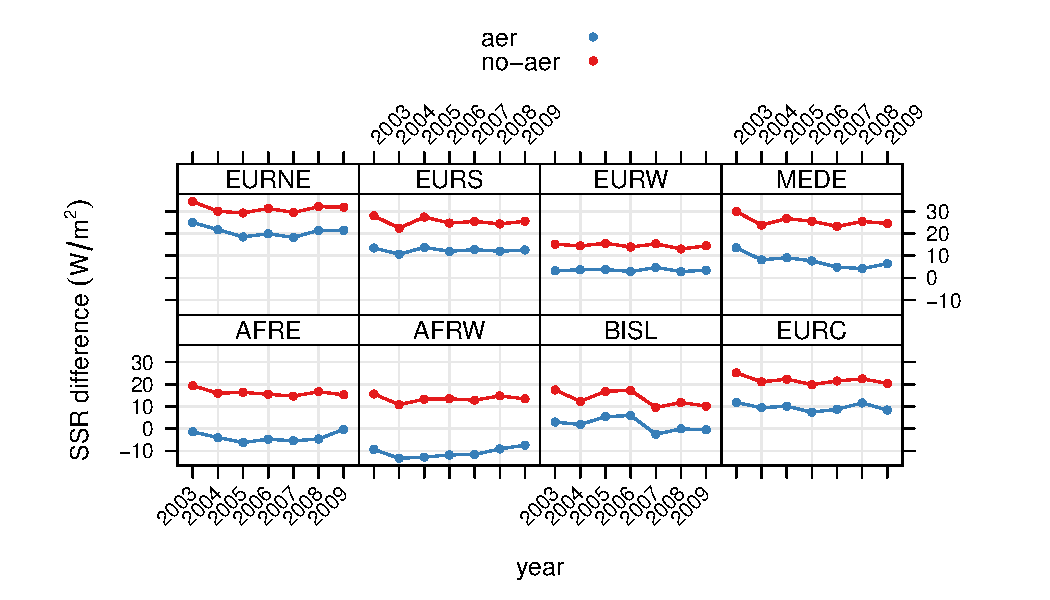
\includegraphics[width=1\textwidth]{figs/capitulo6/dif_model_sat_zonas.pdf}
\caption{Difference in shortwave solar irradiation, SSR $\si{\watt\per\metro\squared}$, between simulations and the satellite aggregated by areas defined in figure \ref{fig:mapapral} in the period 2003-2009.}
\label{fig:figura4}
\end{figure}

In order to calculate the impact on photovolaic production, shortwave solar irradiation, SSR, from the climate model simulations and the satellite dataset is used as an input of the photovoltaic model. For a fixed typology of the panels, the difference between simulations with respect to the satellite dataset as input, in the mean of daily productivity for each month, is represented in figure \ref{fig:ciclosFixed}. The productivity is defined as the energy production per unit of power installed  $\si{\kilo\wattpeak}$.

In general, The NO-AER simulation gives more production than the AER and the satellite, overestimating the PV power potential. Climate model simulations, AER and NO-AER, differ more from satellite PV production output in winter months, whereas in summer months, AER and satellite are close to each other, except form the EURNE region. This area is the most biased area of the model in comparison with the satellite, perhaps due to a bias in the cloud cover.

The regions from North Africa, AFRE and AFRW, are slightly different from the rest with a roughly constant bias curve of the the annual cycle, therefore the difference in PV production between summer and winter months is lower due to the mean latitude of the area. Besides, for these areas, the AER simulations give in summer month lower PV production values than the SAT and the NO-AER, which is not the case in the rest of the regions.

The EURS area is the one with largest amplitude between winter and summer months. For April and May, the AER simulations has small difference with the satellite simulation.

\begin{figure}[h!]
\centering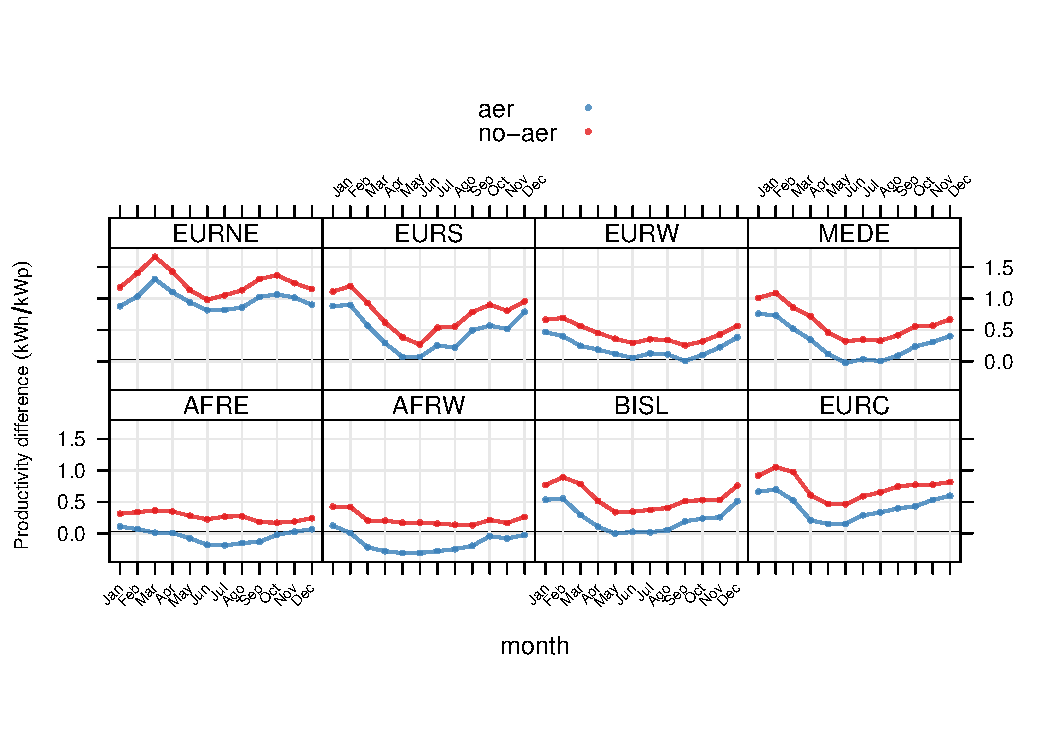
\includegraphics[width=1\textwidth]{figs/capitulo6/diferencia_mesesFIXED.pdf}
\caption{Annual cycle of daily energy productivity  $\si{\kilo\watthour\per\kilo\wattpeak}$ differences by area for the AER simulation and NO-AER simulation with respect to the satellite as inputs of the PV model, considering fixed panels.}
\label{fig:ciclosFixed}\end{figure}

\subsection{Impact of aerosols by tracking type}

\subsubsection{Mean behavior. Period 2003-2009}

In addition to the absolute difference in PV productivity between AER and NO-AER, the relative difference between simulations is presented in this section, showing the relative impact in each case. It allows us to contextualize the loss with respect of the potential of the place.

The difference in yearly PV production between both simulations, for every type of tracking panel, is represented in figure \ref{fig:diferenciaYm}. The spatial pattern shows areas where the aerosols affect more the shortwave solar radiation. Central Europe, Po Valley and the South of the domain, along the African continent coast, are the areas where the differences are more noticeable.

For the fixed panels, the differences are around -150 $\si{\kilo\watthour\per\kilo\wattpeak}$ for some of these areas in annual terms and reaching -200 $\si{\kilo\watthour\per\kilo\wattpeak}$ in the Po Valley, Syria, Iraq and between Algeria and Tunisia.

When the two other tracking systems are considered, the difference between both simulations increases, with values of -300 $\si{\kilo\watthour\per\kilo\wattpeak}$ for the two-axes type over the most affected areas and even higher values like in the south of Turkey. These results are consistent due to the fact that the two-axes and the one-axis tracking systems are more efficient systems to give energy to the generator.

\begin{figure}[h!]
  \centering\begin{subfigure}{1\textwidth}
    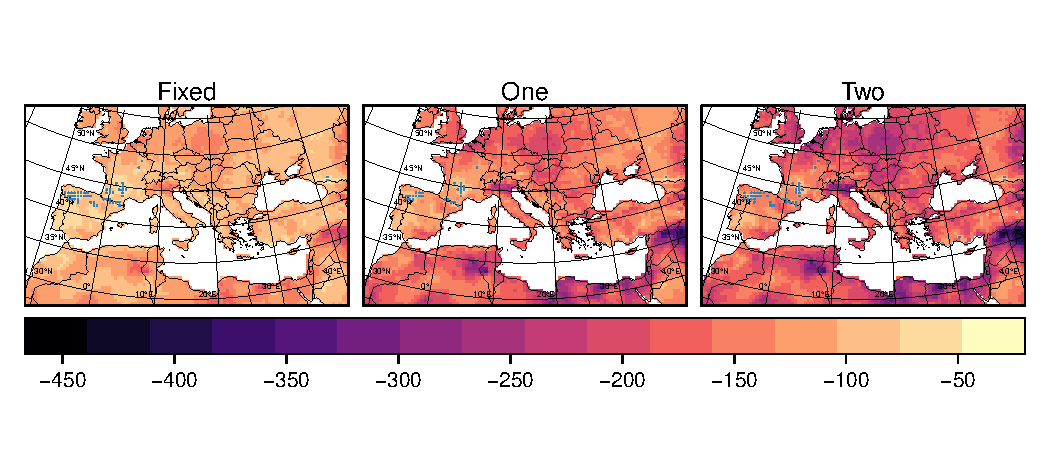
\includegraphics[width=1\textwidth]{figs/capitulo6/dif_aer_no_all_Ym20032009SIGt.pdf}
    \caption{}
    \label{fig:diferenciaYm}
  \end{subfigure}
  %
  \centering\begin{subfigure}{1\textwidth}
    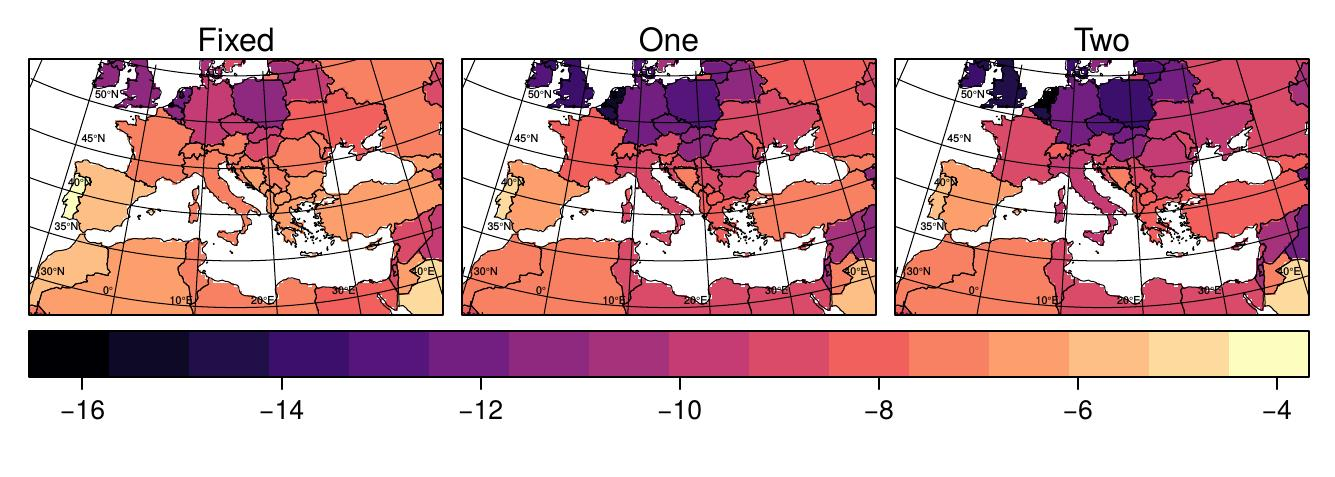
\includegraphics[width=1\textwidth]{figs/capitulo6/byCountry.jpeg}%year_all_bycountry.pdf}%{figs/RelDif_aer_no_all_Ym20032009.pdf}
    \caption{}
    \label{fig:diferenciasRel}
  \end{subfigure}
  %
  \caption{Differences in PV yearly productivity: (a) absolute $\si{\kilo\watthour\per\kilo\wattpeak}$, (b) relative averaged by country (\%); for the period 2003-2009 between AER and NO-AER and for the three different types of tracking. For he non-significant differences, calculated with a 't-test', a point is overplotted for (a)}
\end{figure}

The results of the country averages for the annual productivity are shown in figure \ref{fig:diferenciasRel}. It is shown that the aerosols impact range from $-4\%$ to the PV production to $-16\%$. It can be seen that from the fixed panels to the one-axis, and then to the two-axes tracking type, there is an increase in the productivity losses that is more noticeable in Central Europe, like in Belgium-The Netherlands.

Germany, that have installed a high amount of PV capacity, is affected with values around $-10\%$ of loss for fixed system and more than $-12\%$ for the one-axis and two-axes panels. Thus, some countries with high PV production have moderate losses due to aerosols in relative terms. For countries in the west and south of the domain like Portugal, Spain, Morocco, Jordanian or the extension of Saudi Arabia included in the domain, the relative amount of energy loss is smaller due to its high potential, with differences between $-5\%$ and $-6\%$ for fixed panels and reaching $-8\%$ in some cases for the other types of tracking systems.

\subsubsection{Seasonal cycle}

\begin{figure}[h!]
  \centering
  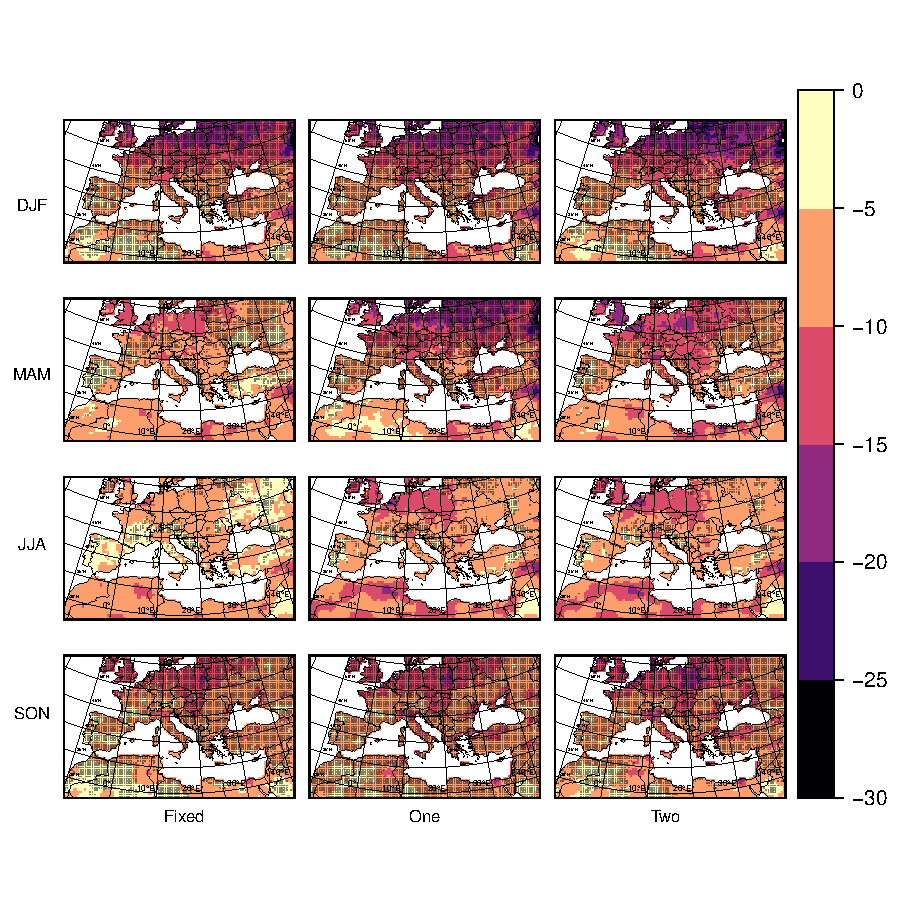
\includegraphics[width=1\textwidth]{figs/capitulo6/RelDif_aer_no_all20032009SIGt.pdf}
\caption{Relative difference (\%) in seasonal PV productivity between both simulation for all type of panels. For the non-significant absolute differences, calculated with a 't-test', a dot is overplotted.}
\label{mapas}
\end{figure}

In seasonal terms spring (MAM) and summer months (JJA) show statistically significant values of the PV productivity difference. For winter (DJF) and Autumn (SON), there are few significant areas, mostly located at the south of the domain, in the African continent. An exception can be found for fixed panels in winter, with significant zones in Europe with values above $-10\%$, like the Po Valley or British Islands. 

The spatial pattern for the spring season shows higher values in Central-Europe, in specific countries like Poland, Belgium and The Netherlands, or British Islands, and in northern parts of Syria and Iraq. Maximum values in these areas, range from an impact higher than $-10\%$ for fixed panels to around $-15\%$ for the two axes tracking type. Almost the whole African part of the domain shows significant differences, with impact values above $-5\%$ and local values reaching more than $-10\%$ between Algerya and Tunisia and in areas of Lybia or Egypt. 

Summer months have higher loads of aerosols over the Mediterranean. For fixed panels, only a few areas in north Africa, Middle East and north-western Europe show values with a loss higher than $-10\%$. One-axis tracking enlarge the extension of areas with a decrease higher than $10\%$ and some areas with more than $-15\%$ appear in Belgium and The Netherlands, Algeria and Syria-Iraq border. Also some smaller areas appear with PV production losses above $-15\%$ within the above mentioned areas. Between the one-axis and the two-axes tracking type, there are no substantial differences in the spatial pattern but maximum values reach in these cases $-17\%$ to $-20\%$ in the same areas.

Significance is not clearly linked to the magnitude of the relative difference in productivity. High relative differences in DJF and SON in central and northern Europe are not significant, due to the high climate variability in these areas and seasons, whereas lower relative differences in spring in Africa and in summer in southern and eastern Europe are mostly significant. The fact that JJA changes are significant over most of the domain explains the statistical significance of most yearly differences (figure \ref{fig:diferenciaYm}), due to the high contribution of summer to the yearly production and yearly interannual variability (see e.g. \cite{Gil2015}).


\subsection{Long-term trends. Period 1980-2012}

The impact of long term trends of solar shortwave on PV production can be illustrated with the results of the simulations of the brightening period over Europe. The simulation including the aerosols dataset, NAB13, and the decreasing trend in sulfur aerosols, TREND, is able to reproduce the observed positive trend in SSR \citep{Nabat2014}.

As a compromise between the lifetime of a PV plant and the length of the simulation, two 15-year periods (at the beginning and end of the simulated period) are evaluated as a proxy for a PV project and the potential amount of energy that can be obtained during such a project. A fixed system is selected for the panels.

The relative difference between the accumulated energy obtained by a 15-year project between 1997-2012 and energy obtained by a 15-year project between 1980-1995 can be seen in figure \ref{fig:trends}.

\begin{figure}[h!]
  \centering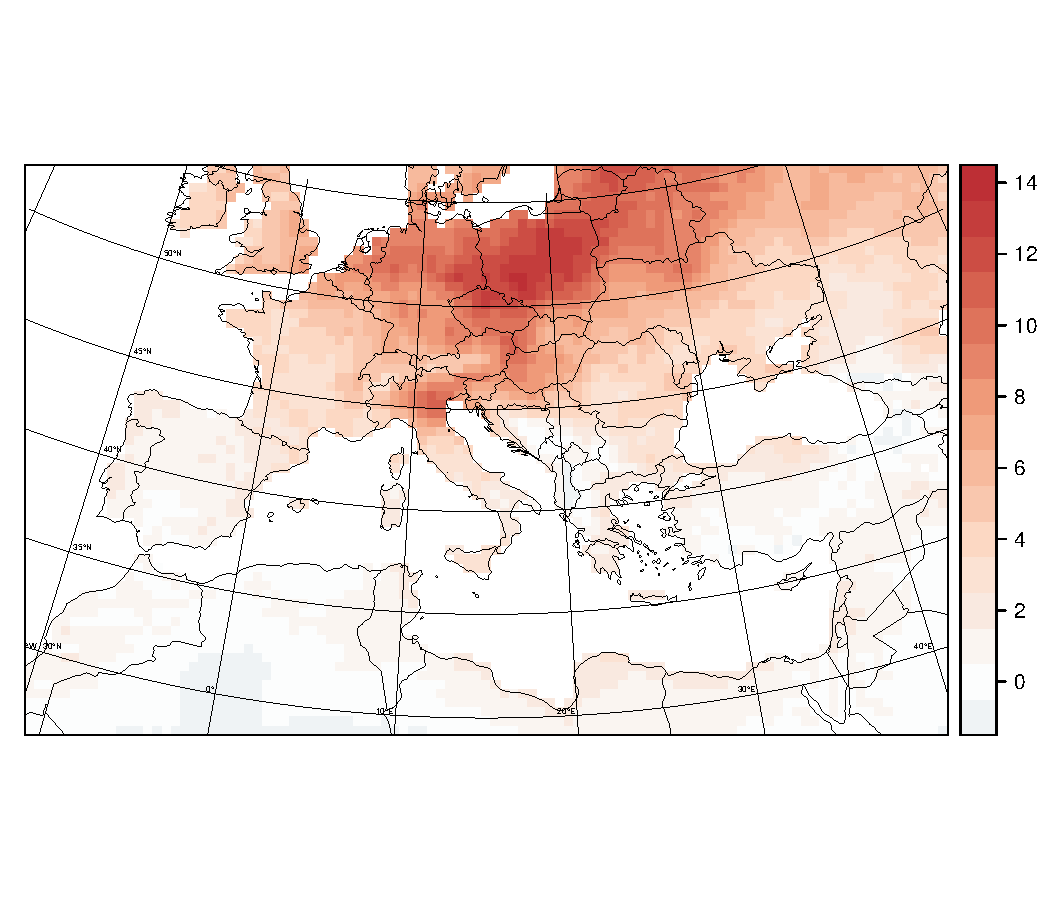
\includegraphics[width=0.7\textwidth]{figs/capitulo6/DifferencesRelativesinPVtciclo15.pdf}
\caption{Relative difference in PV yearly productivity $[\%]$ accumulated for a 15-year period at the end and the beginning of the period: 1980-1994/1998-2012}
\label{fig:trends}
\end{figure}

In Central-Europe the differences in the energy obtained are higher, due to the fact that it is the region where anthropogenic aerosols decrease more. Accumulated over 15 years, an increase higher than 2000 $\si{\kilo\watthour\per\kilo\wattpeak}$ is found for this area. It means that about 10-14 $\%$ more energy can be produced in the lifetime of a PV plant at the end of the period.

These results highlight the impact that environmental policies could have on the PV energy production, showing that anthropogenic aerosols are able to reduce potential PV power of a project significantly. It also illustrates that future evolution of regional anthropogenic aerosols load is likely to influence expected PV production on a given site on the lifetime of a PV plant.

\section{Discussion}
\subsection{Limitations}

The coarse resolution of climate models and their bias in some variables, especially in cloud cover, makes difficult their application for solar resource assessment at local scale in most areas. However, the RCM will evolve to finer resolution and besides, the use of climate models is mandatory for taking into account future climate evolution. They are also relevant tools to perform sensitivity tests allowing to disentangle the driving factors of the resource variability such as aerosols. 

A multi-model approach would be necessary to obtain a more robust answer applying the same methodology to more models but, up to now, aerosols are poorly considered in many RCM, which does not allow that type of study considering actual simulations. 

For the limitations in the PV model, it is important to notice that in the decomposition of SSR and the transposition to the tilted panels, some empirical relationships are used. If components of solar radiation were an output of the RCM, the additional steps for decomposition could be avoided.

It could also be pointed that the spectral decomposition of the SSR reaching the panels would give a better input in order to calculate spectral losses of the PV modules, although for periods longer than a day the spectral effects become less significant \citep{Martin1999}.

In the optical losses, deposition of dust over the generator surface is approximated in the assessment but could be underestimated in desert areas because it is not spatially modeled. That could mean a higher drop in transmittance and final energy production.

The time-scale is also important for the AOD representation. Several processes involving aerosols in the atmosphere are in day to weeks time-scales. We have used a realistic interannual dataset of the AOD that improves the state-of the art used in climate modeling but next studies should go further with an improvement in the aerosols representation. This will include a prognostic scheme of aerosols that allows to study finer time-scales and future scenarios, through a fully-coupled and fully-interactive aerosol-climate model. 
  

\subsection{Implications for the climate services dedicated to the energy sector }

The results show the necessity of considering aerosols in climate simulations used to deliver energy-related climate services. The inclusion of spatio-temporal variability of aerosols in RCMs may change the current estimates of future PV production over Europe \citep{Jerez2015}. An accurate ensemble of models is essential for bridging the gap between services providers and potential users considering that some of the discrepancies between model simulations could come from the aerosols inclusion.

\subsection{PV production data issue}

The scarcity of real power data at PV plant sites is an important issue that has to be overcome in order to improve research in the fields of PV forecasting, climate services or energy modeling. The potential synergies between research institutions and different stakeholders of the energy sector will enhance the PV integration, the management and planning operations as well as the efficiency of the overall system and its development. Not only production data is needed, but also, accurate metadata will be extremely important in order to integrate into the modeling chain important factors such as: days of maintenance activities, cleaning-panel days, installed capacity, electrical characteristics of the PV power plant, among others.

\section{Conclusions}

Two main questions are addressed in this paper: first, the evaluation of the capacity of an RCM to produce reliable estimations of PV production over the Mediterranean area. Secondly, the role of aerosols in PV production using sensitivity tests performed with the RCM. 

It is demonstrated that the use of a RCM as input of a photovoltaic production model is able to reproduce real PV data accurately at monthly time scales for two locations at the domain. Besides, the added value of including aerosols in the simulations is observed over the whole area as the simulation with aerosols shows less bias in SSR than the simulations without aerosols and it is close to the simulated PV using the satellite dataset accross the whole area. 

The results show that the most impacted areas are (with some exceptions) mostly in central Europe, where the lower resource amount in combination with the influence of aerosols gives a significant reduction in potential electricity production. For the annual averaged by country productivity, relative differences are around $-12\%$ for fixed typologies and are seen over Central Europe (Poland and The Netherlands). Differences increase from one axis typology to the two-axes, reaching around $-16\%$ between both simulations in Belgium and around $-13\%$ and $-14\%$ in many countries. In seasonal terms, the loss can reach values of $-20\%$ in some areas for summer months.

In the multi-decadal simulation 1980-2012 a noticeable increase in productivity has been obtained in central Europe as a result of the decreasing trend of anthropogenic aerosols observed from the end of the eighties. This trend has been associated with pollution control measures as well as economic crisis in Western Europe. This result has implications beyond the domain of this study: highly polluted countries like India and China could obtain an increase in PV productivity if pollution control policies are effectively implemented.

The non-negligible impact of aerosols on PV production in the area suggests that the inclusion of aerosols in future scenarios is necessary for solar energy assessment.

\chapter{Future projections of solar resource for photovoltaic applications}

\begin{abstract}

  With the ongoing energy transition, the evolution of renewable energy resources under different climate change scenarios is key for the investors and stakeholders of the energy industry. The possibility of changes in the actual conditions for the operating plants and the projected resources can vary the financial frame of the projects.\\
  
  Although climate models give a robust answer in terms of global warming and other important climate variables, they dissagree in the projected changes of solar resource over Europe. Whereas global climate models, GCM, present a clear positve signal around the mid of XXI century, regional climate models, some studies show a negative anomaly for the same period in RCMs.\\
  
  In this chapter we try to explain the reasons behind the different behaviour focusing on the representation of aerosols in the scenario simulations. We use regional climate models from the EURO-CORDEX project and we focus on the RCP8.5.\\
  
  A fairly pairwise comparison show that regional climate models that include evolving aerosols for the scenarios reverse the sign of the signal in the shortwave solar radiation over Europe or its anomaly is close to zero.\\
  
  We analyse total cloud cover in the regional models simulations and it is not find a clear relationship between the models with aerosols and the anomaly in cloud cover.\\
  
  Due to the clear relationship between sortwave solar radiation anomaly and aerosols evolution, it is necessary to prepare an experiment that is able to give a robust answer in the role of aerosols in terms of shortwave solar radiation projections, which means, that is able to narrow down the uncertainties.\\

  In terms of photovoltaic (PV) potential it has been shown that for RCM with evolving aerosols countries in Central-Europe has a positive anomaly, in contrast with the rest of the RCMs projections. This result revels the impact that the representation of aerosols has in the projections of PV potential for the climate services.\\ 
\end{abstract}

\section{Introduction}

    The generalized increase in the photovoltaic installed capacity in last decades demands the delatiled study of spatio-temporal features of solar resource.\\

  Due to the link between solar energy production and atmospheric variables, there is an increasing concern motivated by the availability of resources under climate change scenarios. Due to that, climate modelling is a key tool to evaluate future energy potential despite of some constrains like its low spatial resolution or cloudiness representation.\\
  
   Although variability of solar radiation are mainly due to changes in cloudiness, in clear days other constituents of the atmosphere, mostly aerosols, decrease the amount of energy reaching the generator surface. Because of its geographical situation, the Euro-Mediterranean area is one of the most influenced areas by natural and anthropogenic aerosols comming from different sources, affecting the spatio-temporal distribution of solar resource.\\

   Different CMIP5 simulations with different GCMs have been evaluated to assess the photovoltaic potential under climate change conditions (wild et al.) and projecting an increase over Europe. However, later studies using regional climate models (Jerez et al. Bartok) have shown an opposite behaviour, an overall decrease in shortwave solar radiation and photovoltaic potential in the same area.\\

   The added value of regional climate modeling against global simulations lies on the better representation of local features that can not be solved with coarser models. However, the increase in resolution has lead to a simplification of other processes in order to not compromise the computational time. Many regional climate simulations have been done using a very simplistic representation of aerosols content (nabat) and they do not include an evolution of aerosols in future projections.\\
   
   In this work we analyse the projections of photovoltaic potential over Europe for the RCP8.5 scenario using regional climate models simulations from EURO-CORDEX initiative. We classify diferent simulations atending to the aerosol representation in the model and its driving global climate model.\\

   Section \ref{Climate data} describes the regional models and simulations used in the study. In section 3 the the main results are explained and a discussion section followed.\\

\section{Climate data: EURO-CORDEX}

\subsection{EURO-CORDEX}

The EURO-CORDEX (Jacob et. al 2014) initiative started as a 'branch' from the Coordinated Regional Climate Downscalling, CORDEX, whose aim is to provide regional climate simulations in different domains. EURO-CORDEX develops climate projections focused on the European continent at different horizontal resolutions (0.44º, 0.11º). These simulations are driven by different CMIP5 GCMs (Taylor et. al 2012).\\

In table 1 there is the information about the aerosols datasets included in the EURO-CORDEX RCMs. It can be observed that only two RCMs from the EURO-CORDEX database include time-evolution of aerosols: RACMO22e and ALADIN5.3. Each of these RCMs have a different dataset of aerosols for projections. Whereas ALADIN5.3 select the Szopa dataset, RACMO22E uses.\\ 

In this work, the choice for the different simulations has followed the next 'pairwise' principle: firstly, RCMs simulations from the EURO-CORDEX database including time evolving scenarios of aerosols are selected. Then, a family of RCMs simulations driven by the same GCMs is constructed around it. Following these steps, we will obtain several groups of RCMs simulations where each one will be called 'family' with the same driven GCM and with only one simulation including aerosols scenarios. Besides, we consider only the RCP8.5 because changes in SSR will be more noticeable and differences between simulations easily detected.\\ 

**La tabla de la descripción de aerosoles de bartok de los GCM se puede referenciar y hacer la de aerosoles de EURO-CORDEX (o de los modelos que yo utilizo?)

\begin{table}
\caption{\label{tb:families}RCMs from EURO-CORDEX grouped by the CMIP5 GCMs drivers generating the 3 families of simulations studied.}
\footnotesize
\begin{tabular}{>{\raggedrigth}m{3cm}>{\raggedright}m{3cm}>{\raggedright}m{3cm}}
\toprule 
CMIP5 GCM & Institution  & RCM  \tabularnewline
\midrule
 CNRM-CM5 & CNRM & ALADIN5.3 \tabularnewline
&CLMcom&CCLM4-8-17\tabularnewline 
&SMHI&RCA4\tabularnewline
\midrule  
ICHEC-EC-EARTH&KNMI&RACMO\tabularnewline
&CLMcom&CCLM4-8-17\tabularnewline
&SMHI&RCA4\tabularnewline
\midrule  
HadGEM2-ES&KNMI&RACMO\tabularnewline
&CLMcom&CCLM4-8-17\tabularnewline
&SMHI&RCA4\tabularnewline  
\bottomrule
%  \br
\end{tabular}\\
%$^{a}$UK spelling is required; $^{b}$MSC classification numbers are required; $^{c}$titles of articles are required in journal references; $^{d}$Harvard-style references must be used (see section \ref{except}); $^{e}$final page numbers of articles are required in journal references.
\end{table}
\normalsize

\begin{table}
\caption{\label{tb:families}RCMs from EURO-CORDEX and aerosols description.}
\footnotesize
\begin{tabular}{>{\raggedrigth}m{1.3cm}>{\raggedright}m{1.3cm}|>{\raggedright}m{2.2cm}>{\raggedright}m{2.2cm}>{\raggedright}m{2cm}}
\toprule 
Institution  & RCM & description & classes & scenarios \tabularnewline
\midrule
CNRM & ALADIN5.3 & Climatology. Szopa 2013 & 5 classes: sea salt, sulfate,black carbon, desert dust,organic carbon.& evolve with RCP \tabularnewline
CLMcom&CCLM4-8-17& Climatology. Tanré 1984 & 4 classes: sea, land, desert, urban.& no evolution\tabularnewline 
SMHI&RCA4& Parametrization in radiation fluxes & Single integrated class.& no evolution \tabularnewline
KNMI&RACMO&CAM inventory, Lamarque 2010 & 6 classes: sulfate, organic matter, desert dust, sea salt,stratospheric aerosols, volcanic & evolve with RCP\tabularnewline
\bottomrule
%  \br
\end{tabular}\\
%$^{a}$UK spelling is required; $^{b}$MSC classification numbers are required; $^{c}$titles of articles are required in journal references; $^{d}$Harvard-style references must be used (see section \ref{except}); $^{e}$final page numbers of articles are required in journal references.
\end{table}
\normalsize


\section{PV potential}

In order to obtain a projection of the photovoltaic productivity over Europe under cliamte change scenarios, a modeling chain approach is considered. Shortwave solar radiation from different climate simulations is used as an input of a photovoltaic model that will give an estimation of the power output. The complete process is explained in chapter 4.\\

The two steps followed in the modeling process of the photovoltaic output are: first, it is necessary to get solar irradiation that reach solar cells, after that the electrical performance of the system is modeled.\\

The process is described in \ref{cha:methods}. In this case, monthly means of daily solar irradiation are used for the decomposition and transformation to the plane of array. Correlation equations between de diffuse fraction and the clearness index described by Page are aplied.   

\section{Results}

\subsection{Anomalies of SSR and CLT}

The anual mean anomaly of the period 2021-2050 for summer months (JJA) with respect to the reference period 1971-2000 is represented in figures 1 and 2 first for shortwave solar irradiation, SSR, and then for total cloud cover, CLT.\\

\begin{figure}[h!]
\centering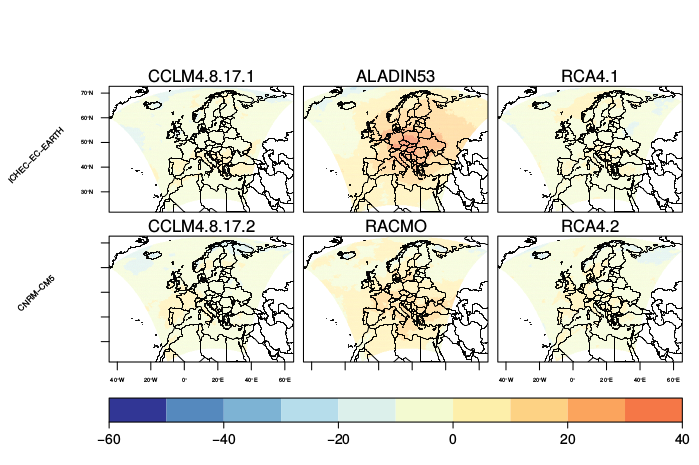
\includegraphics[width=1\textwidth]{figs/capitulo7/ANOMALIAS_JJA_SSR_2050-2021.png}
\caption{}
\label{}
\end{figure}

Anual mean anomaly for summer months shows an increase in Central Europe for climate models with evolving aerosols in scenarios, GCMs and RCMs. In the case of RCMs there are differences in the magnitude of the changes. ALADIN5.3 presents highest anomaly in the mentioned area, which agrees with the anomaly and spatial pattern of aod of this model, as can be seen in figure 3. For RACMO, the aod anomaly has similar spatial pattern but the magnitude is smaller. The same happends with the projected SSR anomalies.\\

The CLT spatial pattern is not complementary with the SSR anomaly map for ALADIN5.3 and RACMO. It means, that the anomaly in SSR is not explained by the anomaly in the total cloud cover. It can be observed, on the contrary that for RCMs with no time-evolving aod the maps are more spatially complementary, as can be also seen in table 3 where values of spatial correlation between both variables are shown. For CM5-ALADIN5.3 and EC-EARTH-RACMO22E the spatial correlation is very low between CLT and SSR and it increase until X and X respectively if AOD is included in the spatial correlation.\\

\begin{figure}[h!]
\centering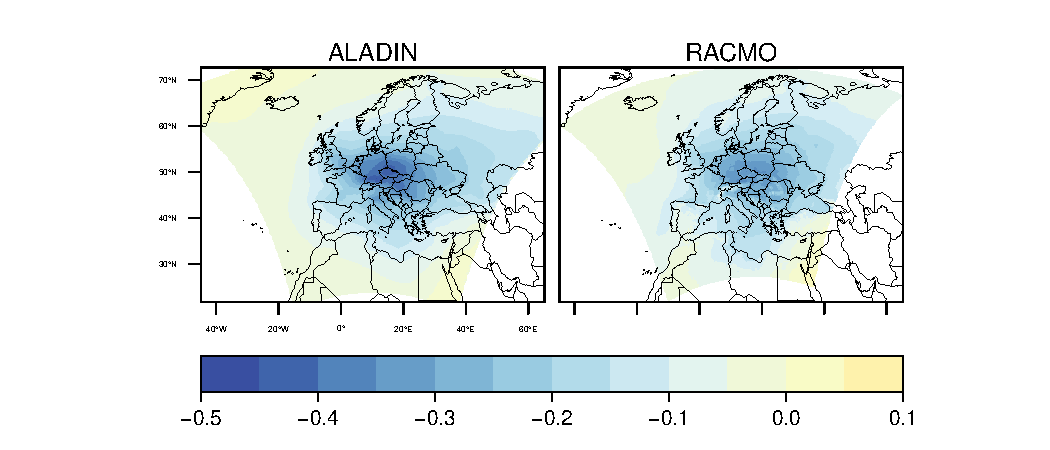
\includegraphics[width=1\textwidth]{figs/capitulo7/ANOMALIAS_JJA_AOD_2050-2021.pdf}
\caption{}
\label{}
\end{figure}

\begin{table}
\caption{\label{tb:spatial correlations}Spatial correlation between SSR,CLT and AOD anomalies maps.}
\footnotesize
\begin{tabular*}{1\textwidth}{@{}llllllll}
\br
CMIP5 GCM & RCM & $\rho_{SSR,CLT}$  & $\rho_{SSR,AOD}$ & $\Delta{SSR}$ & $\Delta{CLT}$ & $\Delta{AOD}$ & $\Delta{PV_{annual}}$\\
\midrule
%  \mr 
CNRM-CM5&ALADIN5.3& -0.26 & -0.94 & 7.15 & 0.60 & -0.10 & 3.5$\%$\\
&CCLM4-8-17& -0.83 & - & -4.17 & -0.15 & - & -2.8$\%$\\
&RCA4& -0.71 & - & -3.55 & 0.21 & - & -2.6$\%$\\
\midrule
% \mr  
ICHEC-EC-EARTH&RACMO& 0.16 & -0.52 & 2.44 & 0.13 & -0.11 & -0.7$\%$\\
&CCLM4-8-17& -0.80 & - & -4.40 & -0.51 & - & -3.9$\%$\\
&RCA4& -0.59 & - & -3.44 & 0.09 & - & -3.6$\%$\\
\midrule  
HadGEM2-ES&RACMO& & & & & &\\
&CCLM4-8-17& & & & & &\\
&RCA4& & & & & &\\  
\bottomrule
%  \br
\end{tabular}\\
%$^{a}$UK spelling is required; $^{b}$MSC classification numbers are required; $^{c}$titles of articles are required in journal references; $^{d}$Harvard-style references must be used (see section \ref{except}); $^{e}$final page numbers of articles are required in journal references.
\end{table}
\normalsize

\subsection{Projected changes in PV production}

The photovoltaic yearly productivity, defined as the power output by the power capacity installed (it is consider a 1 kW system for each grid cell), is calculated for each pixel of land in the domain of EURO-CORDEX. Then, the averaged by country of the relative difference with respect to the reference period 1971-2000 is represented in next figure.

{\color{red} Anomalía para los modelos con aerosoles y los modelos sin aerosoles}

The geographical dependence of the PV anomaly is due to the spatial pattern of SSR anomaly, that is close related with the evolution of AOD in central Europe projected by ALADIN5.3 and RACMO22E. It is important to notice that for the ALADIN53 simulation including aerosols the sign in PV power output anomaly is positive and negative in the other cases. Besides, the RACMO anomaly is close to zero (although negative) whereas the rest of the simulation has the same magnitude order of the anomaly: ~ -2 to -4\%

Uncertainties due to the different AOD datasets used in the two RCMs and in the radiative transfer code of the model difficults the robust answer about the change magnitude. Averaging the results for the non-aerosols simulations and aerosols simulation, we obtain the results in fugure.

\section{Discussion}

To determine the uncertainity in climate projections is one of the main issues in climate science because the information underlyng the simulations is difficult to comunicate. In order to isolate the uncertainity sources in a multi-model workit is necessary to design a sensitivity test for each of the models in the study. Up to now, there are not enough simulations from the EURO-CORDEX ensemble including evolving aerosols and for those that include them, there is not exist the same simulation excluding the aerosols forcing, in order to quantify its impact.

For that reason, this preliminary study, although it highlights very important issues, is the firs step in order to understand the role of aerosols in the RCM projections.

\section{Conclusion}

The study shows that regional climate models with evolving aerosols in the scenarios behaves different than those that has a fixed climatology. In the case of ALADIN53 the sign of the anomaly is reversed, agreeing with the positive signal in PV potential projected by GCMs.

It has been shown also that the anomaly of SSR is not directly linked with CLT anomaly in the case of the RCMs simulation that include evolving aerosols. The spatial correlation between SSR and CLT in this models is very low in comparison to the correlation between SSR and AOD anomaly.

The spatial pattern of the aerosols anomaly impact the future projections of PV differently in each country. The results show a general decresase for RCMs with no-evolving aerosols, more important in higher latitudes. However, for ALADIN53 and RACMO22E simulations the Central-Europe countries present a positive anomaly, which is relevant in terms of energy resource assessment.
% \end{document}